
\documentclass[11pt]{article}

\usepackage{UF_FRED_paper_style}

\usepackage{apacite}
\usepackage{txfonts}
\usepackage{tikz}
\usepackage{amsthm}
\usepackage[capposition=top]{floatrow}
\usepackage[format=plain,
            labelfont={it}, singlelinecheck=false,
            justification = raggedright,
            labelsep = period,
            figureposition=top]{caption}
\usepackage{algorithm}
\usepackage{algcompatible}
\usepackage{algpseudocode}
\usepackage{amssymb}
\usepackage{amsmath}
% for appendix title
\usepackage[title]{appendix}
\usepackage{enumitem} % to remove space between enumerate items

\usepackage[compatible]{algpseudocode}

%for table
\usepackage{tabularx, multirow,booktabs,setspace,caption}
\usepackage{tabularray}
\usepackage[hmargin=1cm]{geometry}


%% for (in)dependence symbols
\makeatletter
\newcommand\multiline[1]{\parbox[t]{\dimexpr\linewidth-\ALG@thistlm}{#1}}
\makeatother

% (in)dependence symbol
\usepackage{unicode-math}

\makeatletter
\newcommand*{\indep}{%
  \mathbin{%
    \mathpalette{\@indep}{}%
  }%
}
\newcommand*{\nindep}{%
  \mathbin{%                  % The final symbol is a binary math operator
    %\mathpalette{\@indep}{\not}% \mathpalette helps for the adaptation
    \mathpalette{\@indep}{/}%
                               % of the symbol to the different math styles.
  }%
}
\newcommand*{\@indep}[2]{%
  % #1: math style
  % #2: empty or \not
  \sbox0{$#1\perp\m@th$}%        box 0 contains \perp symbol
  \sbox2{$#1=$}%                 box 2 for the height of =
  \sbox4{$#1\vcenter{}$}%        box 4 for the height of the math axis
  \rlap{\copy0}%                 first \perp
  \dimen@=\dimexpr\ht2-\ht4-.2pt\relax
      % The equals symbol is centered around the math axis.
      % The following equations are used to calculate the
      % right shift of the second \perp:
      % [1] ht(equals) - ht(math_axis) = line_width + 0.5 gap
      % [2] right_shift(second_perp) = line_width + gap
      % The line width is approximated by the default line width of 0.4pt
  \kern\dimen@
  \ifx\\#2\\%
  \else
    \hbox to \wd2{\hss$#1#2\m@th$\hss}%
    \kern-\wd2 %
  \fi
  \kern\dimen@
  \copy0 %                       second \perp
}
\makeatother
%%%%%%%%%%%%%

% dotted underline
\newcommand{\udensdot}[1]{%
    \tikz[baseline=(todotted.base)]{
        \node[inner sep=1pt,outer sep=0pt] (todotted) {#1};
        \draw[densely dotted, thick] (todotted.south west) -- (todotted.south east);
    }%
}%


%% make cross sign for the table
\newcommand{\tikzxmark}{%
\tikz[scale=0.23] {
    \draw[line width=0.7,line cap=round] (0,0) to [bend left=6] (1,1);
    \draw[line width=0.7,line cap=round] (0.2,0.95) to [bend right=3] (0.8,0.05);
}}


\theoremstyle{definition}
\newtheorem{definition}{Definition}
%use next two lines instead for non-italic alternative
%\newtheorem{preremark}{Definition}
%\newenvironment{mydef}{\begin{preremark}\upshape}{\end{preremark}}

%% ===============================================
%% Setting the line spacing (3 options: only pick one)
% \doublespacing
% \singlespacing
\onehalfspacing
%% ===============================================

\setlength{\droptitle}{-3em} %% Don't touch

\usepackage{authblk} % for adding affiliation

\usepackage{hyperref} % hyperlink
\hypersetup{
    colorlinks=true,
    linkcolor=blue,
    filecolor=magenta,      
    urlcolor=cyan,
    pdftitle={Research Report_Kyuri Park},
    citecolor=black,
    pdfpagemode=FullScreen,
    }
% %%%%%%%%%%%%%%%%%%%%%%%%%%%%%%%%%%%%%%%%%%%%%%%%%%%%%%%%%%
% SET THE TITLE
% %%%%%%%%%%%%%%%%%%%%%%%%%%%%%%%%%%%%%%%%%%%%%%%%%%%%%%%%%%

% TITLE:
\title{Discovering Cyclic Causal Models in Psychological Research 
}


% AUTHOR:
\author[1]{\Large{Kyuri Park \thanks{Corresponding author address: Kyuri Park, Utrecht University, Padualaan 14, 3584 CH Utrecht, The Netherlands. e-mail: k.park@uu.nl}}\\
\large{Supervisor: Dr. Ois\'{i}n Ryan}}
\\
\affil[1]{Department of Methodology and Statistics, Utrecht University}


  
% DATE:
\date{\today}

% %%%%%%%%%%%%%%%%%%%%%%%%%%%%%%%%%%%%%%%%%%%%%%%%%%%%%%%%%%
% %%%%%%%%%%%%%%%%%%%%%%%%%%%%%%%%%%%%%%%%%%%%%%%%%%%%%%%%%%
\begin{document}

{\setstretch{.8}
\maketitle

\noindent\textbf{Research Report: }%
Half of thesis (till Methods section)


\noindent\textbf{Keywords: }%
Cyclic causal discovery; Causal inference; Directed cyclic graph} 


\noindent\textbf{Word count: }%
2500
\\

% %%%%%%%%%%%%%%%%%%%%%%%%%%%%%%%%%%%%%%%%%%%%%%%%%%%%%%%%%%
% %%%%%%%%%%%%%%%%%%%%%%%%%%%%%%%%%%%%%%%%%%%%%%%%%%%%%%%%%%
% BODY OF THE DOCUMENT
% %%%%%%%%%%%%%%%%%%%%%%%%%%%%%%%%%%%%%%%%%%%%%%%%%%%%%%%%%%
% %%%%%%%%%%%%%%%%%%%%%%%%%%%%%%%%%%%%%%%%%%%%%%%%%%%%%%%%%%

% --------------------
\section{Introduction}
% --------------------
A fundamental task in various disciplines of science is to understand the mechanisms, that is causal relations, underlying in the phenomena of interest. In psychology, for example, one of the core questions is how the psychopathology comes about with the network theory of psychopathology positing that mental disorder is produced by a system of direct and mutual causal interactions between symptoms \citep{BorsboomCramer2013}. In practice, empirical researchers often aim to gain insight into these causal relations by fitting statistical network models to observational data \citep{robinaugh2020}. For example, they try to interpret the connections in network models as causal relations (e.g., feeling sad causes insomnia). However, the statistical network models only provide statistical network representation of the underlying system, and it cannot be directly translated into causal relations. In fact, it has been shown that statistical network models are likely to perform poorly for discovering causal relationships, since relations in the network can be produced by unwittingly conditioning on common effects between other variables or induced by unobserved confounding variables. \citep{Ryan2022}.

In the field of causal discovery, causal relations are inferred from observational data based on the patterns of statistical (in)dependencies. \cite{Ryan2022} suggest that network models could in principle be replaced by using purpose-built causal discovery algorithms developed in the field of graphical causal modeling \citep{spirtes_algorithm_1991}. However, the most popular and well-studied causal discovery algorithms assume that causal relationships are acyclic; if X causes Y, then Y does not cause X \citep{Glymour2019}. This is counter to our expectations in psychological settings where the feedback loops are central (ref), which accordingly necessitates the use of \textit{cyclic} causal discovery algorithms \citep{richardson1996}. Cyclic causal discovery algorithms are, however, more difficult to apply and harder to draw inferences from \citep{Bongers2021}. In addition, little research has been done on their performance especially in settings we would expect to encounter in psychological research.

In this paper, we explore the cyclic causal discovery algorithms that are potentially suitable for typical observational psychological data.
We choose three algorithms that can handle cyclic structure: cyclic causal discovery (CCD), cyclic causal inference (CCI), fast causal inference (FCI). The goal of this study is threefold: (a) we want to provide an accessible overview of the set of cyclic causal discovery algorithms; (b) we want to investigate how well each of these algorithms can estimate causal relations by means of a simulation study; (c) we want to test these algorithms by applying them to empirical data.
The paper is organized as follows. ...


% What is the problem we are solving?

\section{Background}

\subsection{Causal Graphical Model} 

A graphical model is a set of multivariate joint distributions that show certain conditional independencies among random variables. Each model is associated with a graph $G = (V, E)$, where $V$ represents a set of vertices (nodes) and $E$ represents a set of edges that encode the conditional independencies between each pair of vertices (ref). 
We use the term causal graphical model to denote a graphical model that describes the causal mechanisms of a system. 
Causal graphical models can capture the probabilistic and causal properties of multivariate distributions, under the two following assumptions.

\begin{enumerate}
    \item \textit{Causal Markov assumption}. A graph $G$ is causally Markov with respect to a joint distribution $P$ over $n$ random variables ($X_1, X_2, ..., X_n$) if it satisfies the recursive factorization property:
$$ P(X_1, X_2, ..., X_n) = \prod_{i}^{n}P(\,X_i \,\,|\,\, pa_{i}^{\mathcal{G}}\,),$$
where $pa_{i}^{\mathcal{G}}$ denotes the \textit{parents} (direct cause) of node $i$ in the graph $G$. This states that a variable $X_i$ is conditionally independent of its non-\textit{descendants} (non-effect variables) given its parents (direct causes). This allows us to read off a set of conditional independencies from graph $G$ such that:  
$$ A \indep_{\mathcal{G}} B \mid C \Longrightarrow X_{A} \indep_{\mathcal{P}} X_{B} \mid X_{C},$$

where $\indep_{\mathcal{G}}$ represents the independence implied by a graph $G$ and $\indep_{\mathcal{P}}$ represents the independence implied by a distribution $P$.


\item \textit{Faithfulness assumption}. It states the reverse of causal Markov assumption. That is, a distribution $P$ is faithful to a graph $G$ if the conditional independencies imply the associated graph structure such that:

$$ X_{A} \indep_{\mathcal{P}} X_{B} \mid X_{C} \Longrightarrow A \indep_{\mathcal{G}} B \mid C.$$
 

\end{enumerate}


\subsubsection{Graph Terminology}

One of the simplest and most well-known causal graphs is \textit{directed acyclic graph} (DAG), also known as \textit{Bayesian networks}, which consists of directed edges without cycles. 
Figure \ref{fig:1} (a) shows the example DAG. 
In the field of graphical models, we use kinship terminology. 
We call a direct cause variable a \textit{parent} (e.g., $X_1$ is the parent of $X_2$), a direct effect variable a \textit{child} (e.g., $X_2$ is the child of $X_1$), an in-/direct cause variable an \textit{ancestor} (e.g., $X_1$ and $X_2$ are the ancestor of $X_3$), and an in-/direct effect variable a \textit{descendant} (e.g., $X_3$ is the descendant of $X_1$ and $X_2$).

It is straightforward how to read off a set of conditional independent relations from a DAG. Again, looking at Figure \ref{fig:1} (a), we can see that $X_1$ and $X_3$ are conditionally independent given $X_2$, as $X_2$ is a mediator. We call such a structure a \textit{chain} ($X_1 \rightarrow X_2 \rightarrow X_3$). $X_3$ and $X_4$ are conditionally independent given $X_2$, as $X_2$ is a common cause, and this structure is called a \textit{fork} ($X_3 \leftarrow X_2 \rightarrow X_4$). Lastly, $X_2$ and $X_5$ are conditionally dependent given $X_4$, as $X_4$ is a collider, and we call it a \textit{collider} structure ($X_2 \rightarrow X_4 \leftarrow X_5$). Following Pearl's \textit{d-separation criterion} (1988, ref), conditional independencies in a causal graph is referred to \textit{d-separation}. For example, in the aforementioned fork structure, $X_2$ \textit{d-separates} $X_1$ and $X_3$, and we state it such that $X_2$ \textit{blocks} the path between $X_1$ and $X_3$. In every distribution, which obeys the causal Markov property, the d-separation implies conditional independence. And if the distribution is faithful to the graph, then conditional independence implies d-separation. 

\begin{figure}[H]
    \centering
        \caption{Example graphical models}
        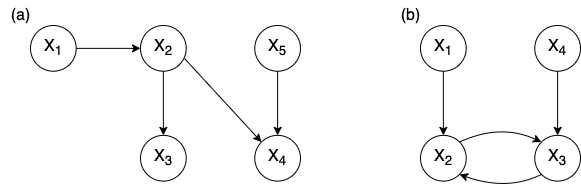
\includegraphics[scale=.5]{figures/DAG_DCG.png}
        \vspace{3mm}
        \caption*{\textit{Note.} (a) is the example directed acyclic graph (DAG). (b) is the example directed cyclic graph (DCG).}
    \label{fig:1}
\end{figure}

\subsubsection{Markov Property} \label{markov_property}
The causal Markov assumption is a commonly made when inferring causal relations from a graphical model. In fact, it entails three Markov properties, which are involved in connecting the graphical structure with the probability distributions: (ref Lauritzen et al,1990)

\begin{definition} [Markov property] \label{def: def1}
Given a directed graph $G$ and a joint distribution $P$, this distribution is said to satisfy
\begin{enumerate}[nolistsep]
    \item \textit{global Markov} property if
    $ A \indep_{\mathcal{G}} B \mid C \Longrightarrow X_{A} \indep_{\mathcal{P}} X_{B} \mid X_{C}$ for all subsets of $A$, $B$, $C$ (also known as the \textit{d-separation criterion}: $A$ and $C$ are d-separated by $B$; $\indep_\mathcal{G}$ refers to d-separation),

    \item \textit{local Markov} property if each variable is independent of its non-descendants given its parents, and

    \item \textit{Markov factorization} property if  $P(X_1, X_2, ..., X_n) = \prod_{i}^{n}P(\,X_i \,\,|\,\, pa_{i}^{\mathcal{G}}\,),$ where $pa_{i}^{\mathcal{G}}$ denotes the \textit{parents} (direct cause) of node $i$ (factorization is in fact equivalent to Global Markov property as long as the distribution over $X$ has a density).
\end{enumerate}
\end{definition}

The elegance of DAG is rooted in the equivalence of these various versions of Markov property. When a DAG satisfies one of these Markov properties, it instantly implies that it satisfies the rest. However, in directed cyclic graphs that is not the case.  
In the directed cyclic graph from Figure \ref{fig:1} (b), it can be observed that global Markov property holds ($ X_1 \indep_{\mathcal{G}} X_4 \mid \{X_2, X_3\} \Longrightarrow X_{1} \indep_{\mathcal{P}} X_{4} \mid \{X_2, X_3\}$), but the
local Markov property is violated as $X_1 \nindep_\mathcal{G} X_4 \mid X_2$ (i.e., $X_1$ is \textit{not} d-separated from its non-descendant $X_4$ given its parent $X_2$). On the contrary, it can be easily seen that all three properties hold in the directed acyclic graph from Figure \ref{fig:1} (a). According to Spirtes (1995), in fact both global and local Markov properties may fail in directed graph with cycles.


\subsection{Structural Causal Model (SCM)} \label{scm}
As the distribution $\mathcal{P}$ may not obey the global Markov property when $\mathcal{G}$ contains cycles, there has to be additional constraints imposed on $\mathcal{P}$ such that we can ensure that the property holds. To do that, first, we need to get the functional form of $\mathcal{P}$. Structural causal models (SCM) (ref Pearl 2009), also known as (non-paramatric) structural equation models (ref Bollen 1989) are widely used to specify the distributions for the causal graphical models. The causal mechanism of a variable $X_i$ is described in SCM by:
$$X_i = f_i\,(\,pa_{i}^{\mathcal{G}}, \varepsilon_i\,),$$
where $f_i$ is a deterministic function depending on the parents of $X_i$ ($pa_{i}^{\mathcal{G}}$), and $\varepsilon_i$ is the random error term.
Spirtes (1995) showed that if $\mathcal{P}$ obeys a linear SCM with jointly independent error terms ($\varepsilon$), then it satisfies the global Markov property with respect to the directed cyclic graph $\mathcal{G}$. 
SCM can represent any causal graphical models, including the non-/linear, and a-/cyclic relationships. Here, we limit the scope of our study to the subclass of cyclic SCMs, where the error terms are normally distributed and relationships between the variables are linear, which are commonly assumed in psychological research. For example, assuming that the graph in Figure \ref{fig:1} (b) conforms to a linear SCM with independent Gaussian error terms, we can illustrate their relations by the linear structural equations as follows:

\begin{equation} \label{eq:1}
  \begin{aligned}
X_1 &= \varepsilon_1,\\
X_2 &= \beta_{21}X_1 + \beta_{23}X_3 + \varepsilon_2,\\
X_3 &= \beta_{34}X_4 + \beta_{32}X_2 + \varepsilon_3,\\
X_4 &= \varepsilon_4,
  \end{aligned}
\end{equation}
where $\boldsymbol{\varepsilon}$ denotes a set of jointly independent Gaussian error terms and $\boldsymbol{\beta}$ denotes a 4 by 4 coefficient matrix.
In the field of structural equation modelling, it is a known fact that the acyclic SCMs, a special subclass of SCMs, are always statistically identified inducing a unique distribution over the variables. However, the linear SCM with cycles are not always statistically identified (ref. Bollen \& Pearl, 2012), which hinders drawing inferences from the models (not sure about this part!!). 

\subsection{Causal Discovery Primer}
Although we encounter various theoretical complications in the cyclic models, we cannot settle for acyclic models especially when the true underlying causal system is believed to contain feedback loops. Despite the difficulties, there has been methods developed for discovering cyclic causal structures using sample data (ref. Richardson, Sprites, Eric).
As previously explained, all causal discovery methods assume the causal Markov property along with the faithfulness to connect the causal graphical structure with the conditional independencies in the data (Geiger, Verma, \& Pearl, 1990).

When considering only observational data (no intervention), there are two principal causal discovery methods: \textit{constraint-based} and \textit{score-based} method. Constraint-based methods focus directly on the connection between graphs and implied independencies. They aim to discover the set of causal graphs that imply exact (conditional) independencies found in the observed data by performing a sequence of conditional independence tests. Score-based methods, on the other hand, compare models on the basis of some measures of model fit (e.g., BIC) and aim to find the globally optimal scoring model. Score-based methods are less developed for the case of possible cycles, and therefore in this paper, we mainly focus on the constraint-based methods.

Constraint-based methods largely work in two steps. The first step is estimating the \textit{skeleton} of the graph $\mathcal{G}$ (undirected version of the underlying graph) based on the fully-connected graph (see Figure \ref{fig:2} (a)). And the second step is orienting as many edges as possible. For example, if we have Figure \ref{fig:1} (b) as our true causal model, a constraint-based method first estimates the skeleton based on the statistical independence relations; if two variables are found independent conditioning on any subsets of the remaining variables (e.g., $X_5 \indep $($X_1, X_2, X_3$)$,\, X_1 \indep X_3 \mid X_2,\, X_1 \indep X_4 \mid X_2, \, X_3 \indep X_4 \mid X_2$, etc.), the edge between the two corresponding variables is removed (see Figure \ref{fig:2} (b)). Secondly, in the orientation step, it looks for a \textit{collider} structure (e.g., $X_2 \nindep X_5 \mid X_4$), which induces conditional dependency that enables us to discern the cause/effect variable. One thing to note is that the resulting graph (Figure \ref{fig:2} (c)) is not identical to the original true graph $\mathcal{G}$ as the two edges between $X_1 - X_2$, and $X_2 - X_3$ remain undirected. As shown in Figure \ref{fig:3}, there are in fact three DAGs (including one true DAG) that can be drawn from the resulting graph from Figure \ref{fig:2} (c). These DAGs are called \textit{Markov equivalent} as they have the same skeleton and collider structure, meaning that they imply the same statistical independencies (i.e., same d-separation relations hold). Figure \ref{fig:2} (c) that represents the \textit{Markov equivalent set} of DAGs is called \textit{completed partially directed acyclic graph} (CPDAG). See Figure \ref{fig:4} for the summary of the constraint-based approach to causal discovery.


\begin{figure}[H]
    \centering
        \caption{Steps of constraint-based method}
        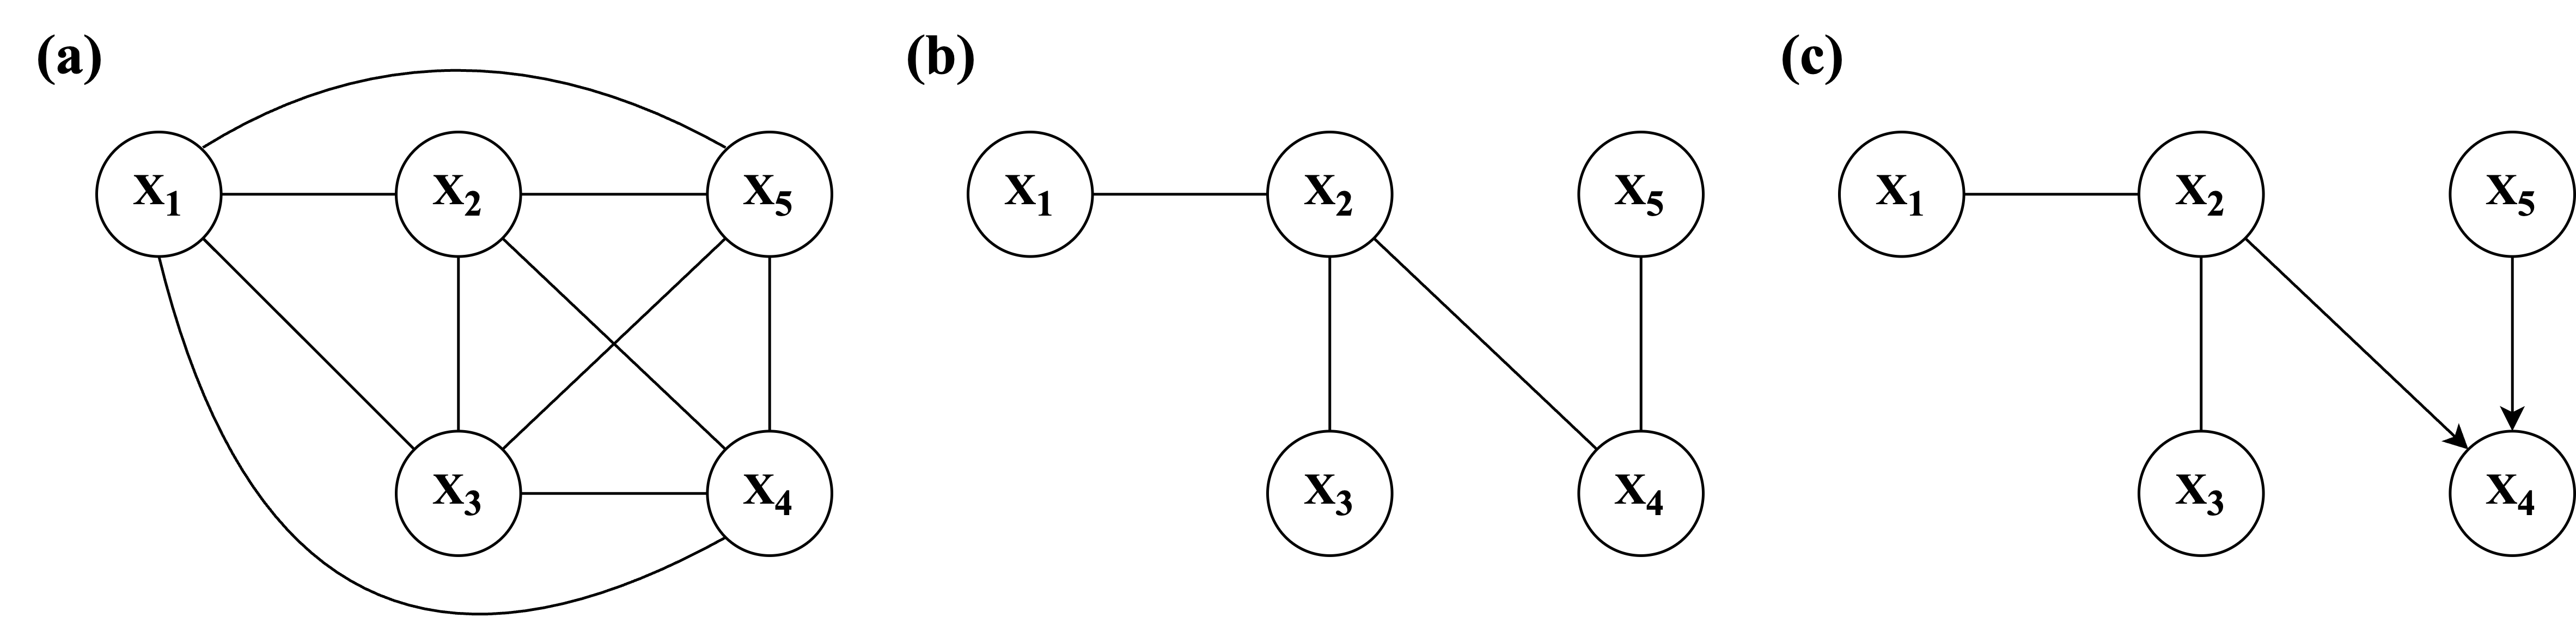
\includegraphics[width=1.0\textwidth]{figures/constraintstep.png}
        \vspace{3mm}
        \caption*{\textit{Note.} (a) is the fully connected graph (starting point). (b) is the \textit{skeleton} (after step 1). (c) is the resulting \textit{CPDAG} (after step 2).}
    \label{fig:2}
\end{figure}

\begin{figure}[H]
    \centering
        \caption{Markov equivalence set of DAGs}
        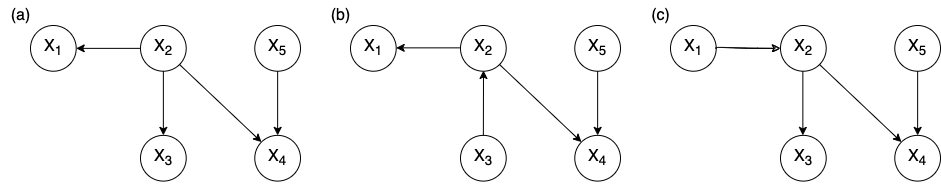
\includegraphics[width=1.0\textwidth]{figures/dag_equiv.png}
    \label{fig:3}
\end{figure}



\begin{figure}[H]
    \centering
        \caption{Summary of constraint-based causal discovery procedure}
        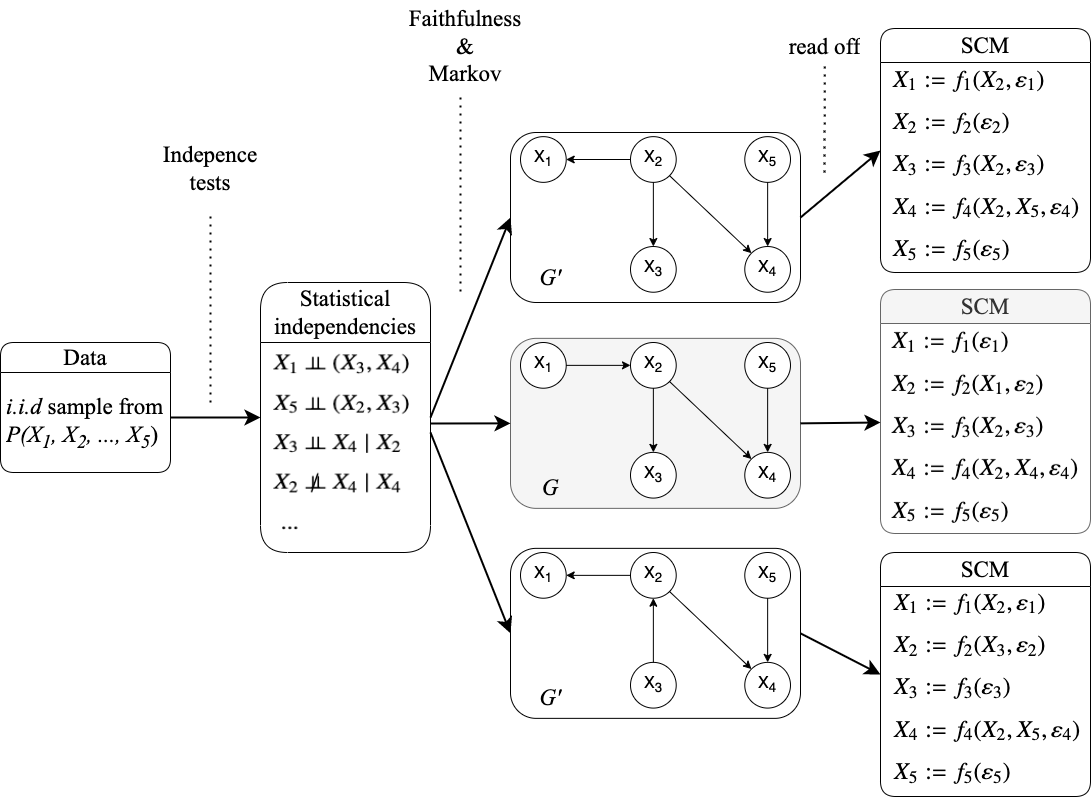
\includegraphics[width=1.0\textwidth]{figures/CB_summary.png}
        \vspace{1mm}
        \caption*{\textit{Note.} The figure summarizes constraint-based approach for causal discovery. It first performs independence tests. The found statistical patterns imply a graph structure by faithfulness and Markov assumption. Often the graph is not uniquely identifiable and results in different graphs $\mathcal{G'}$ including the true graph $\mathcal{G}$ (i.e., Markov equivalent set). Based on the resulting graphs, we can write the underlying SCM equations.}
    \label{fig:4}
\end{figure}


This illustrates the general difficulty of causal discovery based on the observational data. That is, there are numerous causal graphs representing different causal structures (i.e., SCMs), which are all consistent with the observed statistical independencies. Typically, constraint-based methods are unable to identify the unique underlying causal graph, but an equivalence set of graphs. All the constraint-based causal discovery methods for \textit{cyclic} models also work under this fundamental two-step procedure and share this limitation of identifying only the equivalence set instead of the one true graph. However, they differ in several critical aspects: \textit{a}) the assumptions made (e.g., \textit{causal sufficiency}: no latent variable/no confounding), and \textit{b}) the representation of equivalence set of graphs. In what follows, we will introduce three different cyclic causal discovery methods and demonstrate how they work.


% \begin{itemize}
%     \item What is a causal graphical model?
%     \begin{itemize}
%         \item Nodes, edges, meaning of edges. Represents a \textit{Structural Causal Model}; non-parametric causal model.
%         \item Also, mention that this is used in different fields for different reasons
%         \item Probably here: Parents, ancestors, descendants terminology
%     \end{itemize}
%     \item Graphs relate causal relations (in the form of the structure of the graph) to statistical dependencies. Can be seen as representations of joint densities
%     \begin{itemize}
%         \item Example, start with a DAG (three/four variable, but don't yet explain what DAG means)
%         \item explain causal <-> statistical relation using basic d-seperation rules (collider vs confounder vs mediator)
%     \end{itemize}
%     \item More formally, 3 Markov Properties (and what they are)
%     \item Generally, people limit the types of causal graph / model they consider to be acyclic. Directed Acyclic Graph. Briefly/intuitively, why: Easier to deal with! All three markov properties hold. 
%     \begin{itemize}
%         \item [Maybe:] It's also easy to see why DAGs are easier to deal with if we make the connection to linear SEM models, which we can consider to be a very special case of a structural causal model (ref bollen pearl paper 8 myths). There we know that not all cyclic models are statistically identified, which means that, even if we have a cyclic causal model and data on all the variables in the model, performing effect estimation and inference may be practically very difficult.
%     \end{itemize}
%     \item However, in many settings, it may not be appropriate to limit ourselves to DAGs as causal models. Specifically, if we believe that our causal system contains feedback loops! (connection to substantive / psych network world). In that case, we need to deal with cyclic causal models. Moreover in many situations, while we believe that cycles might be present in the underlying causal graph, we don't actually know what the causal graph is. In fact, in many situations, we are explicitly aiming to \textit{learn} the causal graph from a given dataset. In order to do this, researchers might try to use \textit{causal discovery methods} developed for cyclic causal graphs
% \end{itemize}

% \subsection{Causal Discovery Primer}

% \begin{itemize}
%     \item Causal discovery is... (using empirical data to try to recover the causal graph)
%     \item There are many different methods/approaches for causal discovery. If observational data only, then many methods can be described as constraint based or score based methods. Constraint methods use patterns of conditional independence to infer the causal graph, while score based methods look for the "best fitting" model (or so)
%     \item In general, causal discovery from observational data is a difficult problem. The primary reason for this is that, given a particular dataset, there are typically many different causal models which are consistent with the obesrved statistical information. 
%     \begin{itemize}
%         \item Explain constraint based method in general. List all statistical independnece relations. Show how (preferably with the same example as used above), different causal graphs are consistent with those statistical dependencies.
%     \end{itemize}
%     \item Ok, so, we  can see from the example that we haven't learned \textbf{the} causal graph. But, if we are willing to make certain assumptions, then we have learned \textbf{something} about the graph. What are those assumptions. In this case
%     \begin{itemize}
%         \item Faithfulness (brief explanation)
%         \item No unobserved Latent variables
%         \item Let's say it's a DAG too
%         \item Under these assumptions, we can see that, while we don't know the direction of direct causal relationshpis, we did learn about the \textit{presence} or \textbf{absence} of direct parental relationships;
%     \end{itemize}
%     \item More formally, we would say that constraint based causal discovery methods are typically unable to identify \textit{the} underlying causal graph, but instead an \textit{equivalence class} of graphs, that is, a collection of causal graphs that imply the same statistical independence (and so, the same d-seperation) statements. In the previous example we basically showed on an intuitive level the PC algorithm, which identifies an equivalence class of DAGs under the assumptions described above, and represents these with a CPDAG (blah blah)
%     \item Apart from this one shared characteristic (that you identify an equivalence class of some sort), a number of different constraint based causal discovery methods for cyclic models exist. These methods differ critically in many ways, but most importantly in terms of a) the assumptions, such as confounding or no confounding, under which those methods work, and b) how much they can learn about, and in turn how they represent, the equivalence class of possible underlying causal graphs. In what follows we are going to take a brief survey of two different cyclic causal discovery methods and how they work.
% \end{itemize}

\section{Methods}

We consider three different causal discovery algorithms in this paper: cyclic causal discovery (CCD), fast causal inference (FCI), and cyclic causal inference (CCI). Table \ref{tab:1} summarizes the set of assumptions made and the resulting output by each of the algorithms.

\renewcommand{\tabularxcolumn}[1]{>{\centering\arraybackslash}p{#1}}
\renewcommand{\arraystretch}{1.3}

\begin{table}[ht]
\caption{Overview of algorithms.}
\label{tab:1}
\begin{tabularx}{\textwidth}{p{5cm}*{3}{X}}
\toprule
 & CCD & FCI & CCI \\

\midrule
Causal Markov & \checkmark & \checkmark & \checkmark \\
Faithfulness & \checkmark & \checkmark & \checkmark \\
Acyclicity & \tikzxmark & $\textendash ^a$ & \tikzxmark\\
Causal sufficiency & \checkmark &  \tikzxmark &  \tikzxmark \\
Linearity &  \checkmark & \tikzxmark &  \checkmark \\
Independent errors & \checkmark & \checkmark & \checkmark\\
Output & PAG$^b$ & PAG & PAAG$^c$ \\
\bottomrule

\end{tabularx}

\bigskip
\small\textit{Note}. $^a$ FCI is originally designed assuming acyclicity, but in a recent research it has been proposed that it performs comparably well in the cyclic setting \citep{mooij_classen2020}. $^b$ PAG stands for partial ancestral graph. $^c$ PAAG stands for partially-oriented MAAG (maximal almost ancestral graph).
\end{table}


\subsection{The CCD Algorithm}

Cyclic causal discovery (CCD) is a relatively simple causal discovery algorithm for cyclic models, as it assumes that the causal graph may contain cycles but there are no latent common causes (i.e., unobserved variables that are the cause of at least two observed variables) (ref. Richardson). Given the assumption of no latent variables and a linear SCM with independent Gaussian error terms (as discussed earlier in section \ref{scm}), CCD algorithm can represent the cyclic causal structure (d-separation relations in $\mathcal{G}$) generated by distribution $\mathcal{P}$ with the asymptotic correctness.

\subsubsection{Output Representation: Partial Ancestral Graph (PAG)}
Previously, we showed how to estimate \textit{CPDAG}, which represents the Markov equivalent set of DAGs. Here, we aim to find a directed \textit{cyclic} graph (DCG) and to represent the Markov equivalent set of DCGs we employ the \textit{partial ancestral graph} (PAG). (ref. Richardson). Like a CPDAG, a PAG also provides only \textit{partial} information on directions of the relations (i.e., some edges remain undirected) as there are many equivalent graphs exist based on the found statistical patterns. However, a PAG represents \textit{ancestral} relationships, instead of parental relationships. The motivation behind ancestral graph is that as the local Markov property does not generally hold in cyclic graphs (as shown in section \ref{markov_property}), the algorithm cannot estimate the parental relationships directly. 
To represent the equivalent set of cyclic graphs, we need a richer formalism than typical directed graphs. A PAG consists of a set of vertices, edges, and a set of \textit{edge-endpoints} that are drawn from $\{ \circ, -, >, < \}$. $*$ is a so-called meta-symbol that indicate one of the four possible edge-endpoints. In addition, a pair of edge-endpoints can be connected by either solid underlining or dotted underlining. 

\begin{definition} [PAG] \label{def: def2}
$\Psi$ is a PAG for directed cyclic graph $\mathcal{G}$ iff:
\begin{enumerate}[nolistsep]
    \item There is an edge between $A$ and $B$ in $\Psi$ iff $A$ and $B$ are d-connected in $\mathcal{G}$ given all subsets of the remaining vertices.
    
    \item If there is an edge $A -* B$ in $\Psi$, it means $A$ is an ancestor of $B$ in every graph in the equivalent set, $Equiv(\mathcal{G})$.

    \item If there is an edge $A *\rightarrow B$ in $\Psi$, it means $B$ is \textit{not} an ancestor of $A$ in $Equiv(\mathcal{G})$.

    \item If there is a solid underlining $A *-* \underline{B}*-*C$ in $\Psi$, then $B$ is an ancestor of (at least one) $A$ or $C$ in $Equiv(\mathcal{G})$.

    \item If $A \rightarrow B \leftarrow C$, the arrowheads at B can be joined by a dotted underlining $A \rightarrow \udensdot{B} \leftarrow C$, iff $B$ is \textit{not} a descendant of a common child of $A$ and $C$ in $Equiv(\mathcal{G})$.

    \item Any edge-endpoints that are not marked in one of the aforementioned ways, are left with a circle: $\circ-*$.
    
\end{enumerate}
\end{definition}

\subsubsection{Steps of CCD algorithm}
CCD algorithm consists of 6 steps.

In step 1, it estimates the skeleton based on conditional independence patterns. When it finds a conditional independence, it records the variable that d-separate two vertices as a $\mathbf{Sepset}$ of the corresponding d-separated vertices. 

In step 2, it searches for the collider structure. When it finds a collider such that $A \rightarrow B \leftarrow C$, it records $B \notin \mathbf{Sepset}\langle A, B \rangle$. If it detects no collider in a triplets $A *-*B*-*C$, then it adds a solid underline  $A *-* \underline{B}*-*C$ and records $B \in \mathbf{Sepset}\langle A, B \rangle$.

In step 3, it checks for any additional long-range d-separation relations in each triplet $\langle A, B, C \rangle$, where \textit{(i)} $A$ is not adjacent to $B$ or $C$, \textit{(ii)} $B$ and $C$ are adjacent, and \textit{(iii)} $B \notin \mathbf{Sepset}\langle A, C \rangle$. When such $\mathbf{Sepset}$ exists, CCD can orient the edge between $B$ and $C$ such that $B \leftarrow C$ given that $A \nindep B \mid \mathbf{Sepset}\langle A, C \rangle$. (\textit{Being adjacent} means there is an edge between two vertices). 

In step 4, it searches for the $\mathbf{Supset}$, which is a d-separating set including the collider variable. Recall that if we have $A \rightarrow B \leftarrow C$ with $A$ and $C$ being not adjacent, then every set d-separating $A$ and $C$ does not contain $B$. But in a cyclic graph, $A$ and $C$ can be d-separated given a set contains $B$. When CCD finds such set, it records it as a $\mathbf{Supset}\langle A, C \rangle$. 

In step 5, it searches for the quadruplets (i.e., four ordered vertices $\langle A, B, C, D \rangle$) that contain two colliders such that \textit{(i)} $A \rightarrow \udensdot{B} \leftarrow C$ and \textit{(ii)} $A \rightarrow D \leftarrow C$ or $A \rightarrow \udensdot{D} \leftarrow C$. If $B$ and $D$ are adjacent in such a structure, CCD then orients the edge between $B$ and $D$ using the $\mathbf{Supset}$ that is found in step 4.

In step 6, it searches for the quadruplets $\langle A, B, C, D \rangle$ where $A \rightarrow \udensdot{B} \leftarrow C$, while $D$ is adjacent to neither $A$ nor $C$. CCD again uses the $\mathbf{Supset}$ to orient the edge between $B$ and $D$.

For the detailed description of each step of CCD, see Appendix \ref{algCCD}.

%trace CCD
\subsubsection{Trace of CCD algorithm}
Given a conditional independence oracle for $\mathcal{G}$ in Figure \ref{fig:1} (b), the CCD algorithm runs as follows.

\textbf{Step 1.} As $X_1 \indep X_4 \mid \emptyset$, $X_1 \multimapboth X_4$ edge is removed and record $\mathbf{Sepset} \langle A, B \rangle = \mathbf{Sepset} \langle B, A \rangle = \emptyset$.

\textbf{Step 2.} \multiline{As $X_2 \notin \mathbf{Sepset} \langle X_1, X_4 \rangle$, orient $X_1 \rightarrow X_2 \leftarrow X_4$. As $X_3 \notin \mathbf{Sepset} \langle X_1, X_4 \rangle$, orient $X_1 \rightarrow X_3 \leftarrow X_4$.}

\textbf{Step 4.} \multiline{As $X_1 \indep X_4 \mid \{X_2, X_3\}$, orient $X_1 \rightarrow \udensdot{$X_2$} \leftarrow X_4$ and $X_1 \rightarrow \udensdot{$X_3$} \leftarrow X_4$.\\
Record $\mathbf{Supset}\langle X_1, X_2, X_4 \rangle = \{X_2, X_3\}$ and $\mathbf{Supset}\langle X_1, X_3, X_4 \rangle = \{X_2, X_3\}$.}
\vspace{.1mm}

\textbf{Step 5.} \multiline{There is a quadruple such that $X_1 \rightarrow \udensdot{$X_2$} \leftarrow X_4$, $X_1 \rightarrow \udensdot{$X_3$} \leftarrow X_4$, $X_2 \multimapboth X_3$. \\
As $X_2 \in \mathbf{Supset} \langle X_1, X_3, X_4 \rangle$, orient $X_2 \multimap X_3$.\\
As $X_3 \in \mathbf{Supset} \langle X_1, X_2, X_4 \rangle$, orient $X_2  - X_3$.}
\vspace{.1mm}

Note that \textbf{step 3} and \textbf{step 6} do not perform any orientation in this case.

\begin{figure}[H]
    \centering
        \caption{Trace of CCD algorithm.}
        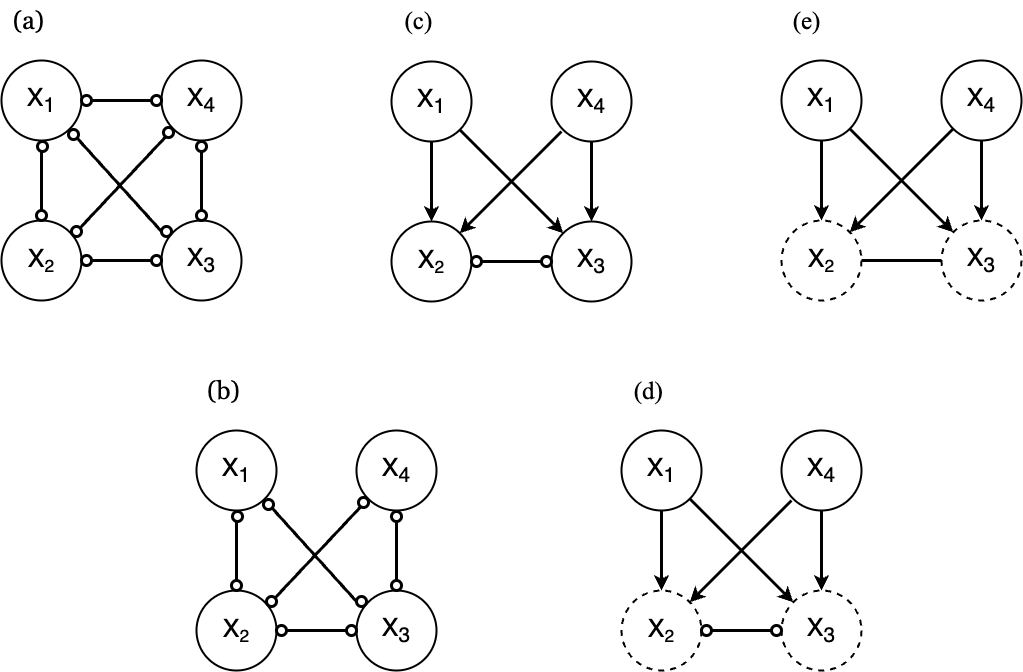
\includegraphics[width=.8\textwidth]{figures/ccdtrace.png}
        \vspace{3mm}
        \caption*{\textit{Note.} (a) is the fully-connected graph, which is the starting point. (b) is the estimated skeleton after step 1. (c) is after the colliders are identified in step 2. (d) is after step 4, where the \textit{Supsets} are identified and correspondingly dotted underline is added. (e) is the final resulting PAG after step 5, where the additional edge is oriented between $X_2$ and $X_3$.}
    \label{fig:5}
\end{figure}

\begin{figure}[H]
    \centering
        \caption{Strategy for CCD algorithm.}
        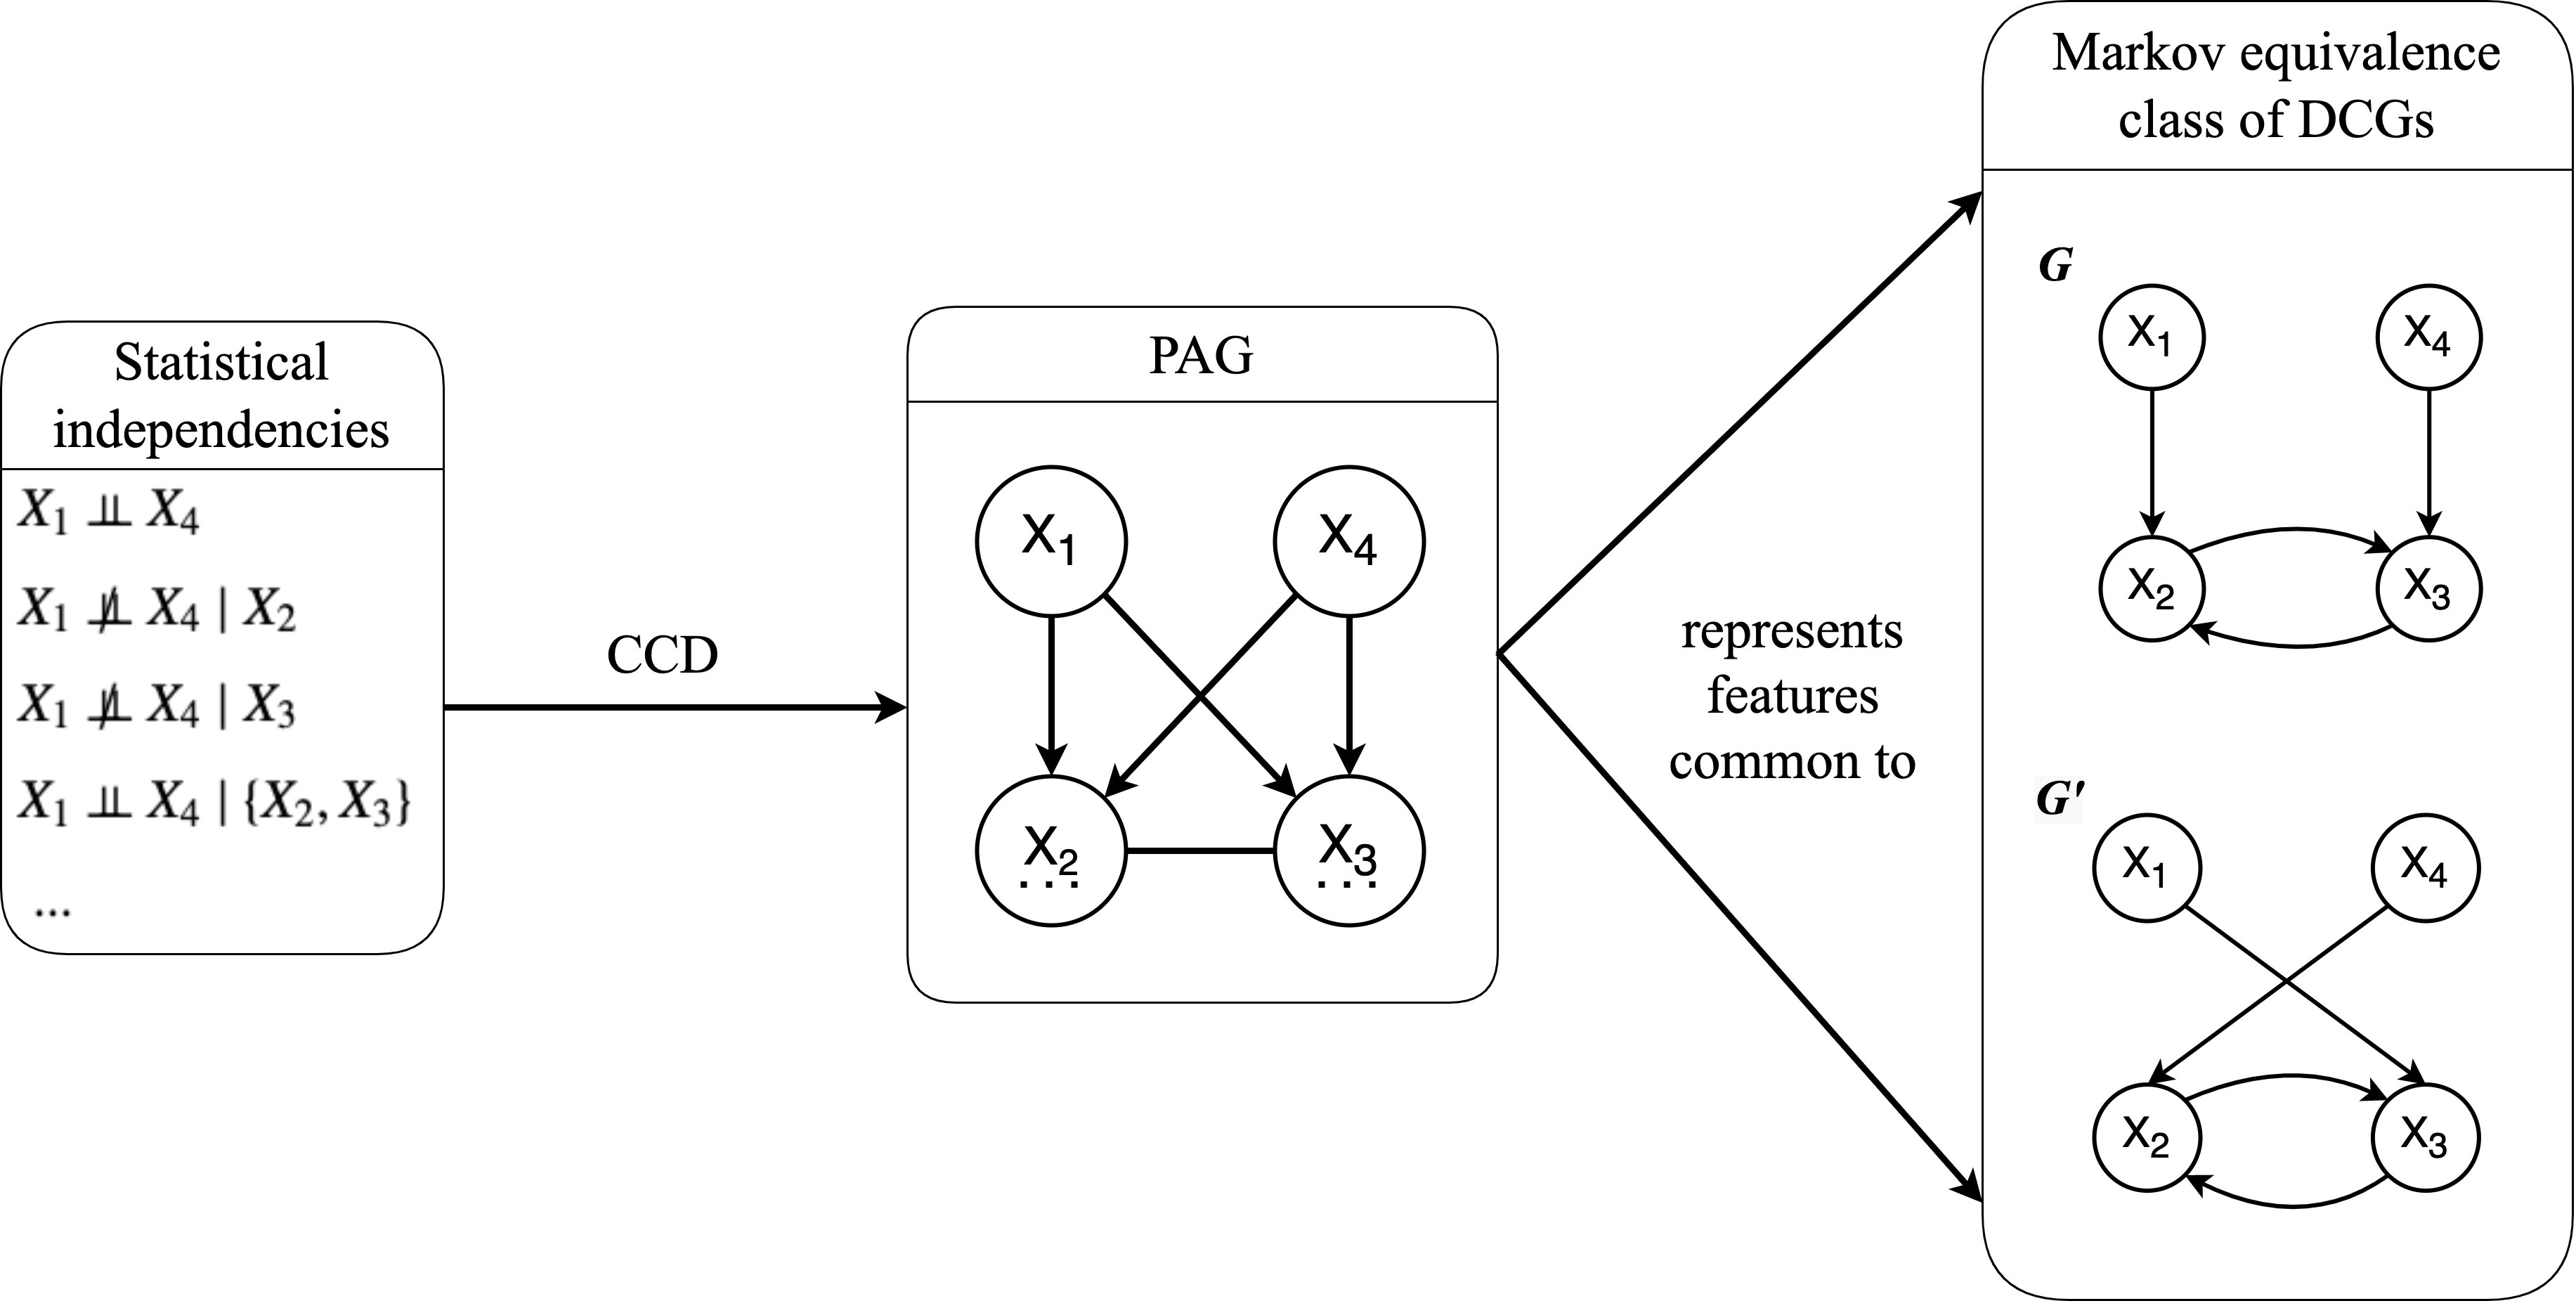
\includegraphics[width=1.0\textwidth]{figures/CCDsummary.png}
        \vspace{1mm}
        \caption*{\textit{Note.} Given the statistical independencies, CCD construct a partial ancestral graph (PAG), which represents features common to all directed cyclic graphs in the Markov equivalence class.}
    \label{fig:6}
\end{figure}


% \begin{itemize}
%     \item Background, what it is.
%     \item Assumption of this method: no latent variables, but we allow cycles
%     \item In the previous section, we could find a method that estimates the CPDAG. For this method, it's trickier; we are typically not able to identify definitively the presence or absence of direct parental relationships - but instead we have to settle for identifying \textit{ancestral} relationships. Give intuition why (pairwise markov property + simple example)
%     \item More formally, we would say that the CCD algorithm identifies an \textit{Ancestral Graph}. Description. Eeven more specifically than that, Richardson describes this as a Partial Ancestral Graph (PAG) (why partial?)
%     \item What edges are allowed in the PAG and what they mean.
%     \item Ok, how does this work. Sketch of the Algorithm. Example with each step applied
%     \item Ok, now how does the PAG represent an equivalence class? Show me the cyclic graphs in the equivalence class
% \end{itemize}




\subsection{Fast Causal Inference (FCI)}

CCD algorithm is shown to be sound (i.e., algorithm makes correct inferences from conditional independencies in $\mathcal{P}$ as long as the assumptions hold (ref Richardson). However, it still comes with a shortcoming. That is, it assumes that there is no latent variables (i.e., causal sufficiency), which is seldom appropriate. Fast causal inference (FCI) algorithm is explicitly designed to handle latent variables in acyclic settings. It relaxes causal sufficiency assumption, while assuming the acyclicity. However, it has been recently proposed that FCI in fact can handle cycles by showing that the accuracy of FCI when having it run on the data generated by a cylic casual model is comparable to its accuracy in the strictly acyclic setting (Mooij \& Classen, 2020). Therefore, here we decide to consider FCI as a possible cyclic causal discovery algorithm and look into it in further detail.

\subsubsection{Output Representation: Partial Ancestral Graph (PAG)}
FCI also employs the PAG to represent the Markov equivalent class of ancestral graphs. The motivation to use ancestral graphs is a bit different from CCD. As FCI allows the possibility that latent variables may exist, using ancestral graphs is suitable since they are closed under marginalization of latent variables (DAGs are not closed under marginalization) (ref. Zhang \& Spirtes, 2005). However, not all ancestral graphs satisfy the global Markov property. Markov property is guaranteed only if an ancestral graph is \textit{maximal}, meaning that every missing edge corresponds to a conditional independence relations. Hence, a PAG that results from FCI represents the set of maximal ancestral graphs (MAGs) and it comes with a slightly different kinds of edge end-points along with its interpretation compared to the PAG from CCD.
The PAG from FCI can have bidirectional edges ($\leftrightarrow$) that represent the presence of latent confounders, while they do not exist in the PAGs from CCD. Additionally, the dotted underlining does not occur in PAGs from FCI. 


\begin{figure}[H]
    \centering
        \caption{Strategy for FCI algorithm.}
        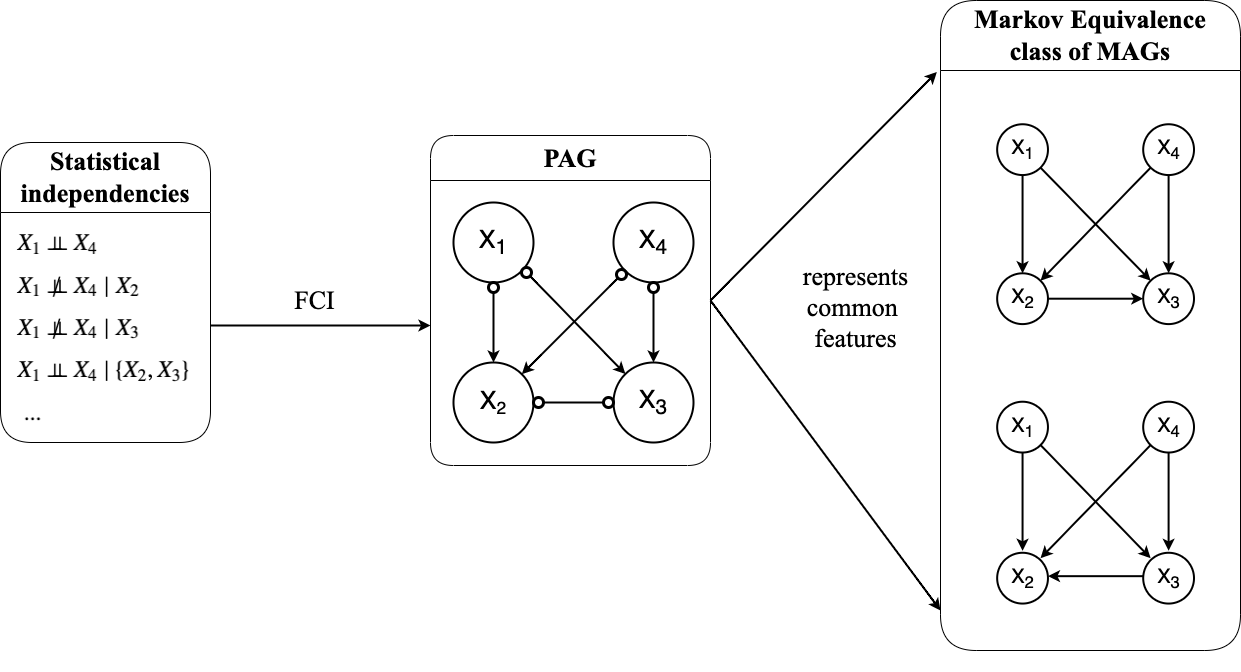
\includegraphics[width=1.0\textwidth]{figures/FCIsummary.png}
        \vspace{1mm}
        \caption*{\textit{Note.} Given the statistical independencies, FCI construct a partial ancestral graph (PAG), which represents features common to all maximal ancestral graphs in the Markov equivalence class.}
    \label{fig:7}
\end{figure}



\subsubsection{Steps of FCI algorithm}
FCI algorithm consists of 4 steps.
Each step of FCI is illustrated using the same example model from Figure \ref{fig:1} (b) as below. 

Like in CCD, it starts with a fully-connected undirected graph (Figure \ref{fig:7} (a)). In step 1, it estimates the skeleton based on the found statistical conditional independencies (i.e., it removes the edge between $A$ and $B$ and records $C$ as a $\mathbf{Sepset} \langle A, B \rangle$ iff $X_{A} \indep_{\mathcal{P}} X_{B} \mid X_{C}$, where $C$ is any subset of $\mathcal{V} \backslash \{A, B\}$). As $X_1 \indep X_4 \mid \emptyset$, $X_1 \multimapboth X_4$ edge is removed and record $\mathbf{Sepset} \langle A, B \rangle = \mathbf{Sepset} \langle B, A \rangle = \emptyset$, which results in Figure \ref{fig:7} (b).

In step 2, it searches for collider structures to start orienting edges. For each triplet $\langle A, B, C \rangle$, if the pair of $A$ and $B$ as well as $B$ and $C$ are adjacent but not the pair of $A$ and $C$ (i.e., $B \notin \mathbf{Sepset} \langle A, B \rangle$), then orient $A \multimapboth B \multimapboth C$ as $A \multimapinv > B < \multimap C$. Given that $X_2 \notin \mathbf{Sepset} \langle X_1, X_4 \rangle$ and $X_3 \notin \mathbf{Sepset} \langle X_1, X_4 \rangle$, orient $X_1 \multimapinv > X_2 < \multimap X_4$ and $X_1 \multimapinv > X_3 < \multimap X_4$, which results in Figure \ref{fig:7} (c).

In step 3, it computes \textbf{Possible-d-sepset} for each pair of vertices (e.g., $\textbf{Possible-d-sepset} \langle A, B \rangle)$, which are the set of vertices that we have not definitely determined to be not in the \textbf{Sepset} of corresponding pairs of vertices (e.g., $\mathbf{Sepset} \langle A, B \rangle$). If we find that $A$ and $B$ are d-separated given any subset $S$ of $\textbf{Possible-d-sepset} \langle A, B \rangle \backslash \{A, B\}$, then we remove the edge between $A$ and $B$, and record $S$ as $\mathbf{Sepset} \langle A, B \rangle$. In this case, there has not been found any subsets of \textbf{Possible-d-sepset} that additionally d-separate a pair of vertices.

In step 4, it further orients the edges using a set of orientation rules iteratively until no more edges can be oriented. In this case, none of the orientation rules is found to be applicable, which results in Figure \ref{fig:7} (c) as the final PAG model. See Appendix \ref{algFCI} for the list of orientation rules including other details of FCI algorithm.





\begin{figure}[H]
    \centering
        \caption{Trace of FCI algorithm.}
        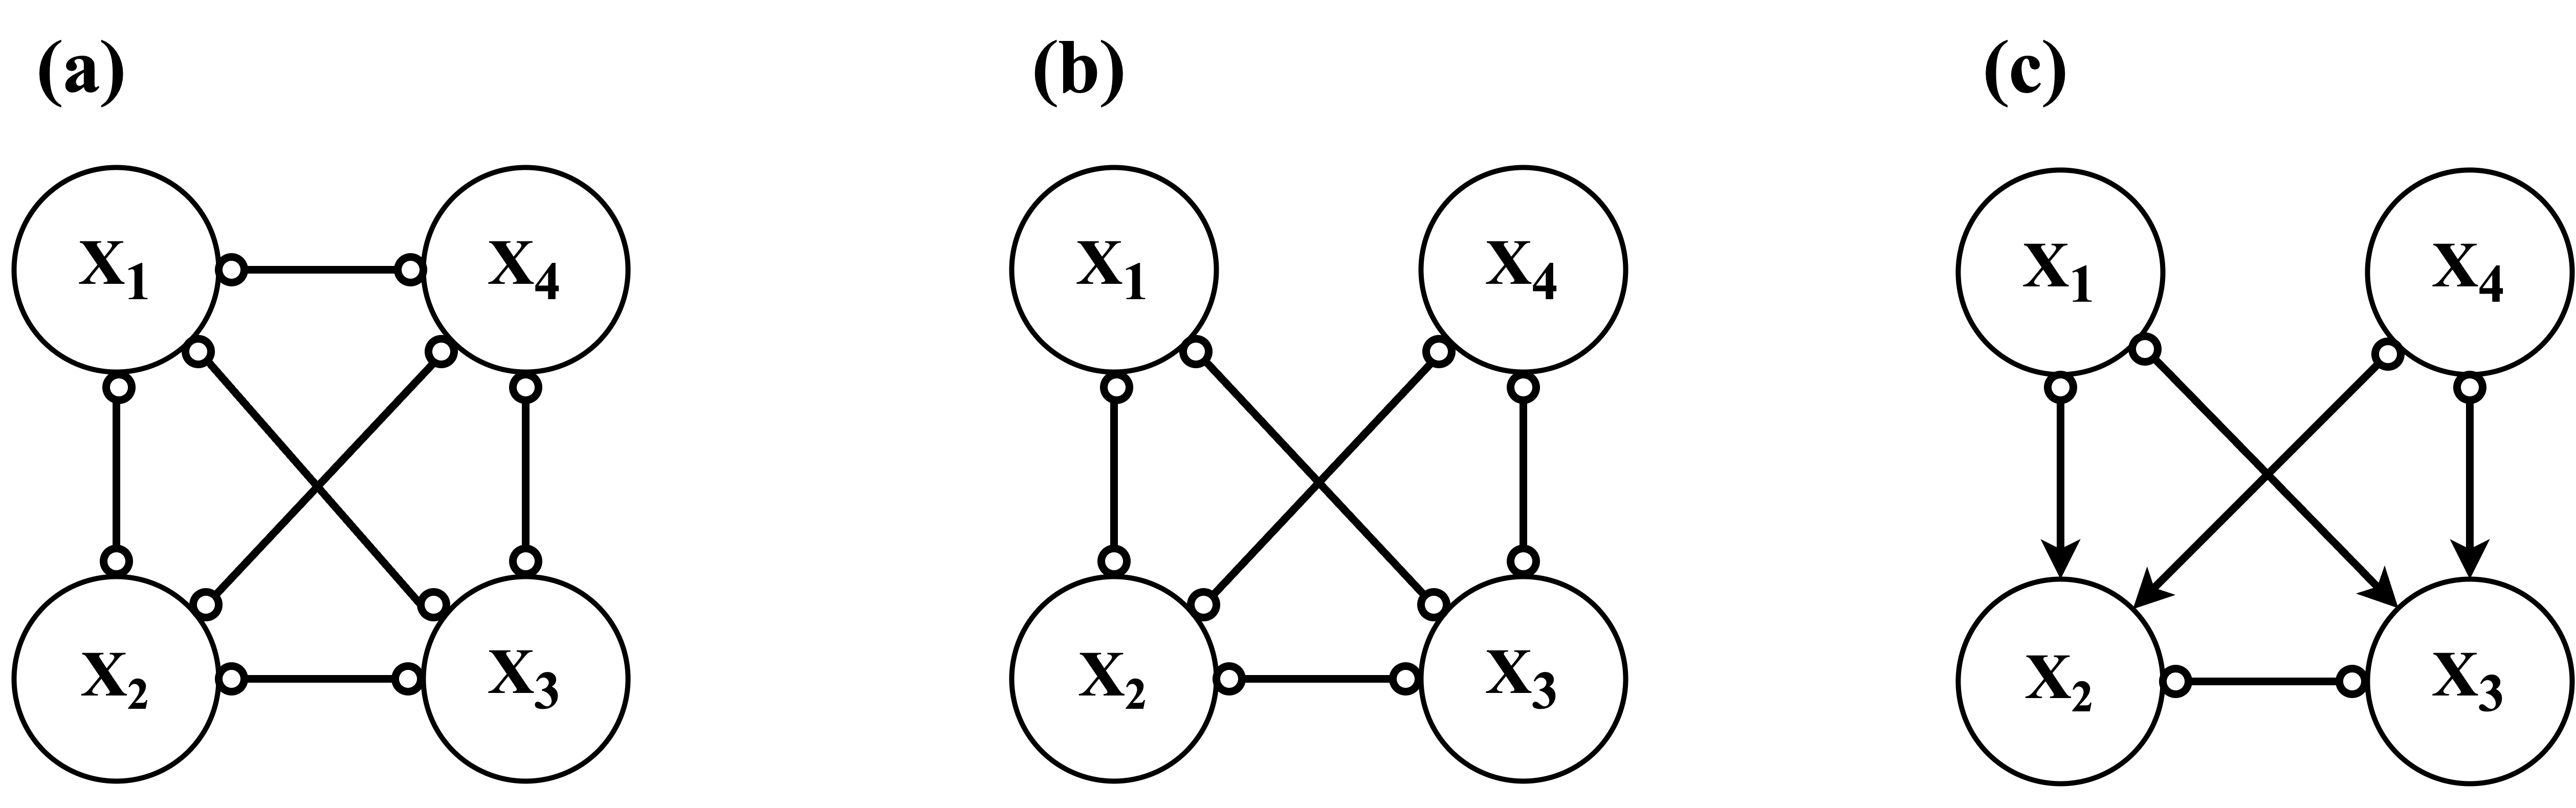
\includegraphics[width=0.8\textwidth]{figures/FCItrace.png}
        \vspace{1mm}
        \caption*{\textit{Note.} (a) is the fully-connected undirected graph, which is the starting point. (b) is the estimated skeleton after step 1. (c) is after the colliders are identified in step 2. No further orientation is performed under step 3 and step 4, and accordingly FCI results in (c) as the final PAG.}
    \label{fig:8}
\end{figure}



\subsection{Cyclic Causal Inference (CCI)}
CCI algorithm is one of the algorithms that can handle cycles, latent variables, and selection bias simultaneously. It could be seen as a combined version of CCD and FCI, considering that it allows cycles while assuming linearity like CCD, and it utilizes maximal ancestral graphs to summarize the directed graphs with latent and selection variables like FCI (ref. Eric).

\subsubsection{Output Representation: Partially oriented MAAG (PAAG)}
While CCI is deemed to be the most general of the considered algorithms in terms of the fact that it can deal with cycles as well as latent variables at the same time, it comes with a relatively limited class of output representation, which is called maximal almost ancestral graphs (MAAG). Unlike a MAG from FCI, a MAAG does not necessarily preserve the d-separation relations, hence called \textit{almost}. Like in a PAG, the resulting output is a \textit{partially oriented} MAAG (PAAG), meaning that it only shows the partially oriented edges, while using circles ($\circ$) to represent the uncertain edge-endpoints. 


\begin{figure}[H]
    \centering
        \caption{Strategy for CCI algorithm.}
        \vspace{1mm}
        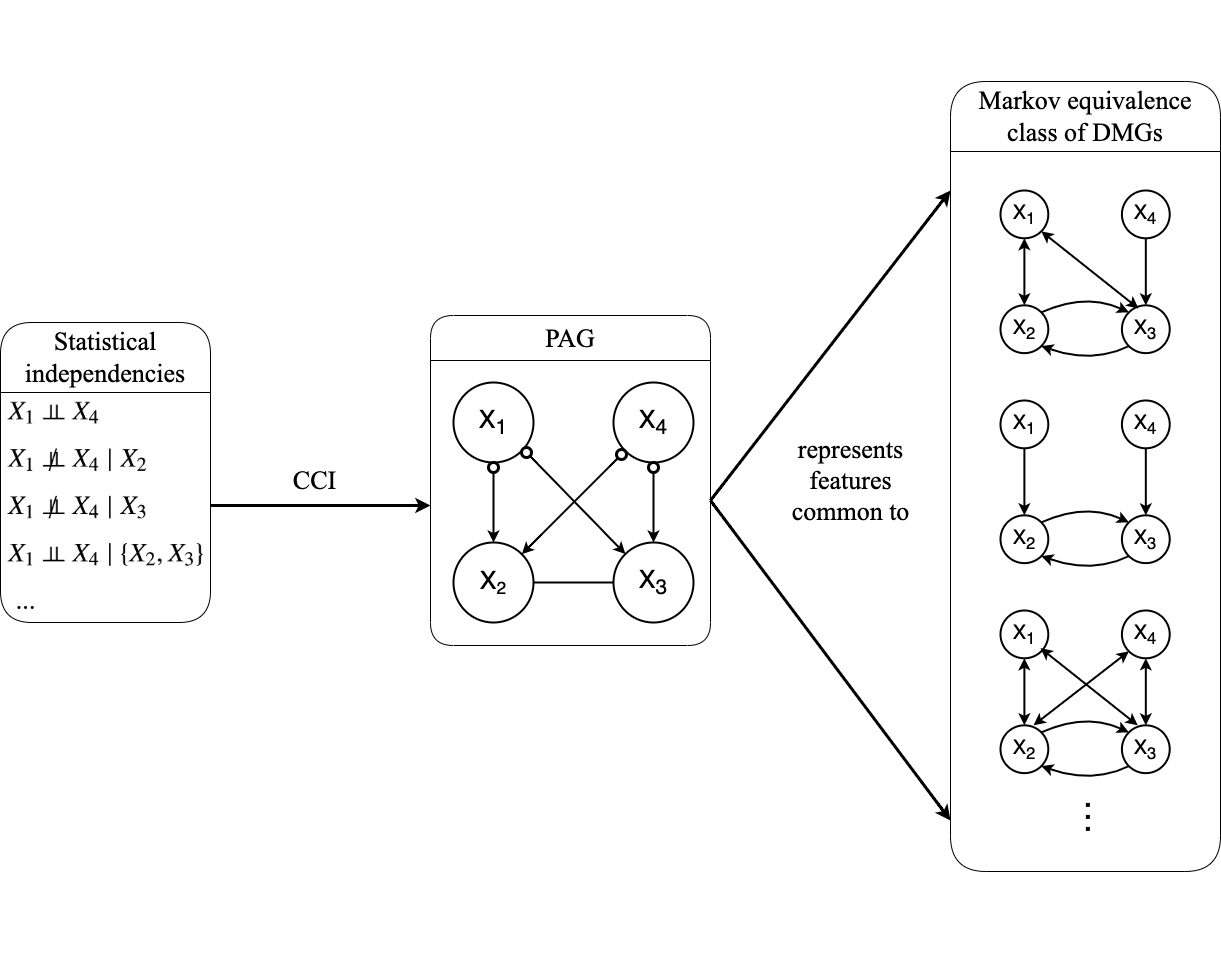
\includegraphics[width=1.0\textwidth]{figures/CCIsummary.png}
        \vspace{1mm}
        \caption*{\textit{Note.} Given the statistical independencies, CCI construct a partially oriented almost ancestral graph (PAAG), which represents features common to all maximal almost ancestral graphs in the Markov equivalence class. Notice that the d-separation relation is not always preserved in MAAG. For example, $X_1$ and $X_4$ are m-connected given $\{X_2, X_3\}$ when $X_1 \indep_{\mathcal{G}} X_4 \mid \{X_2, X_3\}$ in the third MAAG.}
    \label{fig:9}
\end{figure}

\subsubsection{Steps of CCI algorithm}
CCI consists of 7 steps in total. The first two steps are basically identical to the steps of FCI.

Like the other two algorithms, it starts with the fully-connected undirected graph (Figure \ref{fig:10} (a)). In step 1, CCI performs the FCI's skeleton discovery procedure. As it finds $X_1 \indep X_4 \mid \emptyset$, the edge ($X_1 \multimapboth X_4$) is removed (Figure \ref{fig:10} (b)) and it records $\mathbf{Sepset} \langle A, B \rangle = \mathbf{Sepset} \langle B, A \rangle = \emptyset$.

In step 2, it searches for collider structures in the same way as FCI does. Upon finding that $X_2 \notin \mathbf{Sepset} \langle X_1, X_4 \rangle$ and $X_3 \notin \mathbf{Sepset} \langle X_1, X_4 \rangle$, it orients $X_1 \multimapinv > X_2 < \multimap X_4$ and $X_1 \multimapinv > X_3 < \multimap X_4$, which results in Figure \ref{fig:10} (c).

In step 3, it checks for long-range d-separation relations, as it could be the case that two cyclic directed graphs agree locally on d-separation relations, but disagree on d-separation relations between distant variables. The basic reasoning is the same as the step 3 of CCD. In this case, no long-range d-separation set has been discovered and correspondingly no further orientation is performed.

In step 4, it searches for non-minimal d-separation sets, which correspond to the $\mathbf{Supset}$ from CCD algorithm. Here, it finds $\mathbf{Supset}\langle X_1, X_2, X_4 \rangle = \{X_2, X_3\}$ and $\mathbf{Supset}\langle X_1, X_3, X_4 \rangle = \{X_2, X_3\}$.

In step 5 and step 6, it utilizes the found additional d-separation sets from step 4 to orient the edges. In step 5, if finds a quadruple such that $X_1 *\rightarrow X_2 \leftarrow* X_4$, $X_1 *\rightarrow X_3 \leftarrow* X_4$, $X_2 \multimapboth X_3$. Given that $X_2 \in \mathbf{Supset} \langle X_1, X_3, X_4 \rangle$ and $X_3 \in \mathbf{Supset} \langle X_1, X_2, X_4 \rangle$ (as discovered in step 4), it orients $X_2 \multimapboth X_3$ as $X_2 - X_3$, which leads to Figure \ref{fig:10} (d). No further orientation is performed in step 6.

In step 7, it orients the edges further applying a set of orientation rules, which is an extended version of orientation rules of FCI. It finds no applicable orientation rules in this case. See Appendix \ref{algCCI} for the detailed description for each step of CCI.



\begin{figure}[H]
    \centering
        \caption{Trace of CCI algorithm.}
        \vspace{1mm}
        \includegraphics[width=1.0\textwidth]{figures/CCItrace.png}
        \vspace{1mm}
        \caption*{\textit{Note.} (a) is the fully-connected undirected graph, which is the starting point. (b) is the estimated skeleton after step 1. (c) is after the colliders are identified in step 2. (d) is after step 5, where the additional edge is oriented between $X_2$ and $X_3$. No further orientation is performed under step 7 and accordingly CCI results in (d) as the final PAAG.}
    \label{fig:10}
\end{figure}




\subsection{Simulation}

In the following sections, we discuss the data generating process and the specifics of simulation study design. In addition, we will briefly introduce the empirical data on which we test the algorithms.

\subsubsection{Generating data}
To examine the performance of the algorithms that we described in the previous section, we simulate data from the linear cyclic SCMs. The data-generating procedure consists of three steps. First, we specify the structural equations representing the linear cyclic SCM (see Equation \ref{eq:1} for example). Secondly, we draw the values of $\varepsilon$ according to their independent distributions. Lastly, we obtain the values of each random variable $X$ by solving the following system of equations: $\mathbf{X} = (\mathbf{I} - \mathbf{B})^{-1}\mathbf{\varepsilon}$. Note that the equations may not have unique solutions for every cyclic SCM. The necessary condition to have a unique solution is that $(\mathbf{I} - \mathbf{B})$ has to be invertible and in cyclic models, this condition is only met when the absolute values of eigenvalues of $\mathbf{B}$ are all smaller than one, $|\lambda| < 1$ (Eberhardt, Hoyer \& Scheines, 2010). Therefore, we ensure that the specified $\mathbf{B}$ satisfies the aforementioned condition.

\subsubsection{Simulation design}
In the simulation study, we generate data from different types of cyclic models by varying the number of variables (rows of Figure \ref{fig:11}) and density (columns of Figure \ref{fig:11}). We also test the performance under the presence of an unobserved confounder by adding a latent variable ($L_1$ in Figure \ref{fig:11}). Lastly, we vary the sample size across the range we often encounter in psychological network $n \in \{150, 500, 1000\}$, for all considered cyclic models (ref.Cramer\&constantin), which produces a $2 \times 2 \times 2 \times 3$ design; number of variables $\times$ density $\times$ confounder (yes/no) $\times$ sample size.


\begin{figure}[H]
    \centering
        \caption{Simulation settings.}
        \vspace{1mm}
        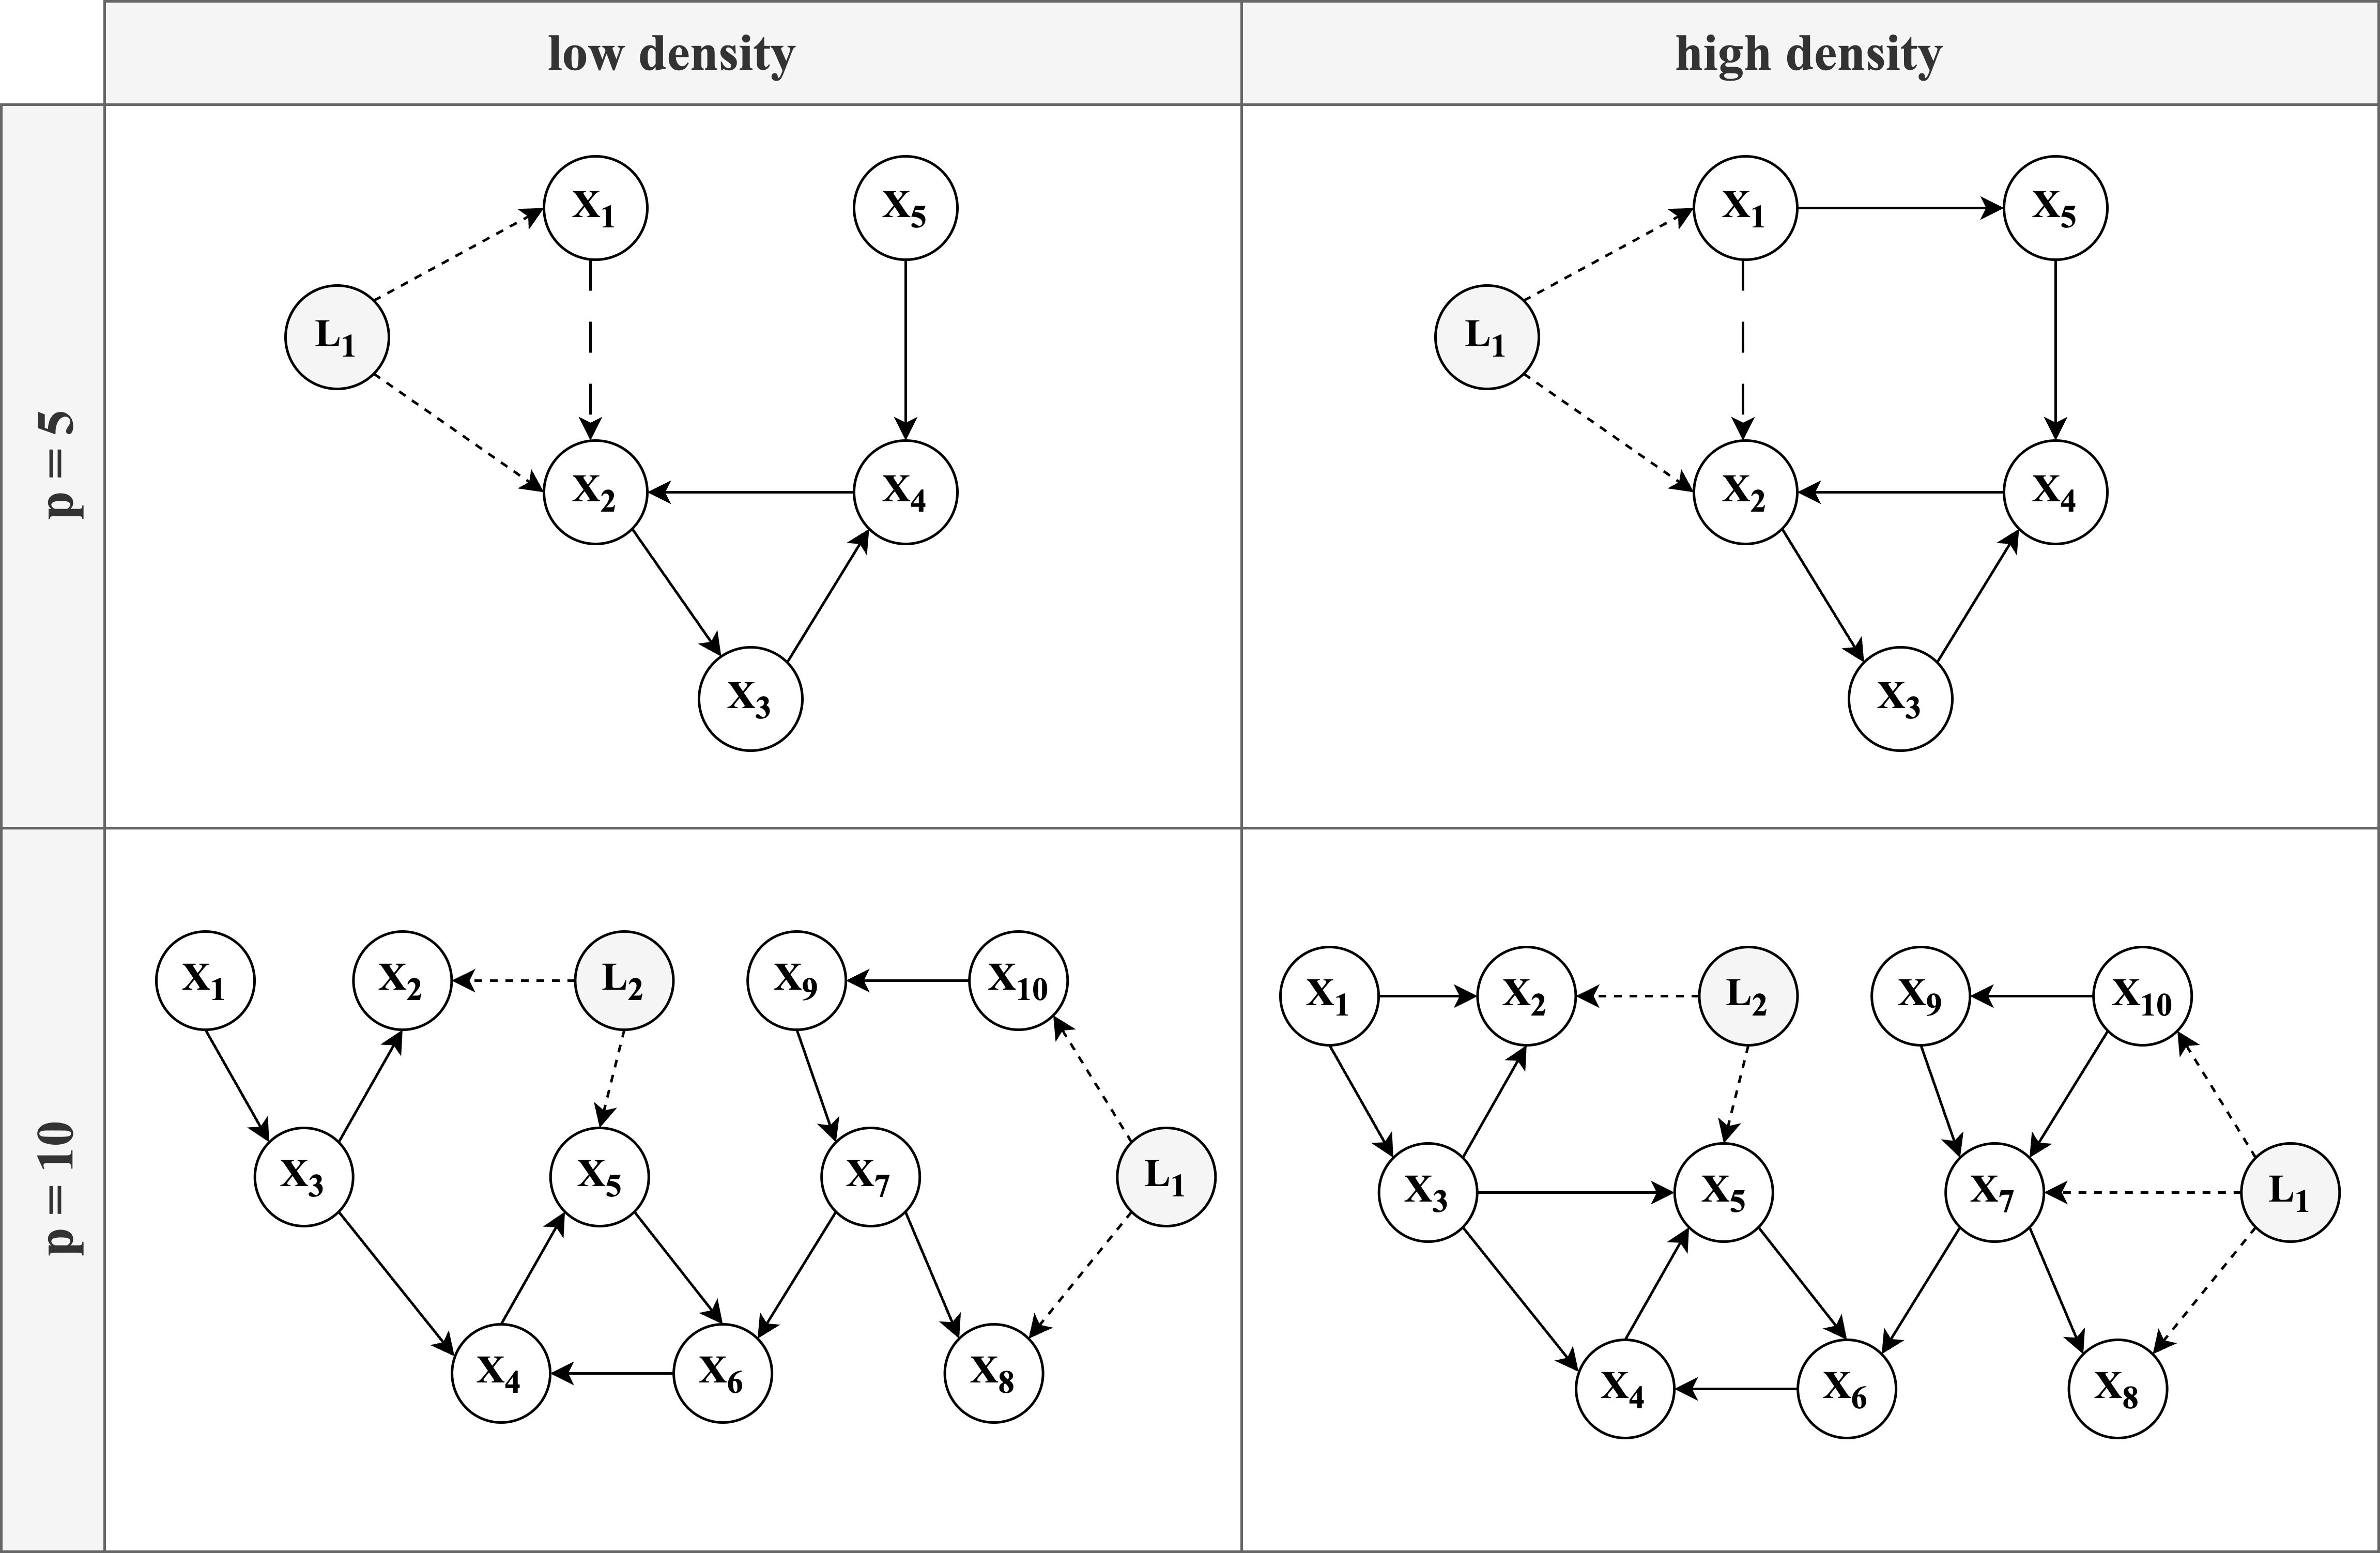
\includegraphics[width=1\textwidth]{figures/simsetting3.png}
        % \vspace{1mm}
        \caption*{\textit{Note.} $p$ is the number of variables in the graph.  $L_1$ is a latent variable.}
    \label{fig:11}
\end{figure}


\subsubsection{Evaluation metrics}
We first assess the algorithms using the average precision, recall, and uncertainty rate. Precision reflects the prediction accuracy (e.g., out of predicted cases, how many are correct), and recall reflects the retrieval rate (e.g., out of true cases, how many are retrieved). There are in total four possible cases for each endpoint in the resulting graph: no endpoint (null), arrow head ($>$), arrow tail ($-$), and circle ($\circ$). Given that circle endpoint implies that the algorithm fails to identify the direction, we compute its uncertainty rate based on the proportion of the circle endpoints occurred in the output. For the other endpoints, we compute the precision and recall, then average them out to evaluate the performance. For example, if we compute the precision and recall for the arrow head, we can compute them such that $Precision =  \frac{a}{a + d + g}$ and $Recall = \frac{a}{a + b + c}$ (see Table \ref{tab:2}).

$$Precision = \frac{\text{True Positive}}{\text{True Positive } + \text{ False Positive}}$$
$$Recall = \frac{\text{True Positive}}{\text{True Positive } + \text{ False Negative}}}$$
$$Uncertainty = \frac{\text{Number of circle endpoint } (\circ)}{\text{Total number of endpoints}}$$


\begin{table}[ht]
\begin{center}
\caption{Confusion matrix.}
\label{tab:2}
\begin{tabular}{@{}cc|ccc@{}}
\multicolumn{1}{c}{} &\multicolumn{1}{c}{} &\multicolumn{3}{c}{\textbf{Estimated endpoint}} \\ 
\multicolumn{1}{c}{} & 
\multicolumn{1}{c|}{} & 
\multicolumn{1}{c}{arrow head ($>$)} & 
\multicolumn{1}{c}{arrow tail ($-$)} &
\multicolumn{1}{c}{\hspace*{4mm} null \hspace*{4mm}} \\ 
\cline{2-5}
\multirow[c]{2}{*}{\rotatebox[origin=tr]{90}{\textbf{True endpoint}}}
& arrow head ($>$)  & \textit{a} &  \textit{b} & \textit{c}   \\[1.5ex]
& arrow tail ($-$)  & \textit{d}   & \textit{e} & \textit{f} \\[1.5ex]
& null  & \textit{g} & \textit{h} & \textit{i} \\[1.5ex]
\end{tabular}
\end{center}
\smallskip
\small\textit{Note}. The circle endpoint ($\circ$) is not counted towards true/false positive/negatives, but used to compute uncertainty rate.
\end{table}

% Or we can just use structural hamming distance (SHD)? It seems it is quite a popular metric to use when comparing the graphs (also pcalg has a function for this). It sounds relatively simple at a glance, but I haven't looked into this in very much detail. 

For the overall performance, we use structural Hamming distance (SHD) (ref.). SHD quantifies the level of differences between two graphs by counting the number of edge insertions, deletions, and direction changes required to move from one graph to the other (true graph). Thus, the large SHD values indicate dissimilarity, whereas small SHD values indicate similarity of the two graphs.



\subsection{Empirical Data}

\section{Expectations}




% \section{Discussion}


% \begin{enumerate}
%     \item Summary
    
%     \item Other interesting things we didn't fully discuss
    
%     \item Outlook
% \end{enumerate}



% \section*{Acknowledgements}


\bibliographystyle{apacite}
\bibliography{references} 

%\bibliographystyle{plain}
%\bibliography{references}




\pagebreak

\begin{appendices}

\section{CCD Details}\label{algCCD}

%% CCD algorithm %%

\begin{algorithm} 
\caption{Cyclic Causal Discovery (CCD)}
 % input
 \hspace*{\algorithmicindent} \textbf{Input:} A conditional independent oracle\footnote{explain orcale} for a distribution $\mathcal{P}$, satisfying global directed Markov property and faithfulness conditions with respect to a directed graph $\mathcal{G}$ with vertex set $\mathcal{V}$. \\

 % output
 \hspace*{\algorithmicindent} \textbf{Output:} A PAG $\Psi$ for the Markov equivalence class $\text{Equiv}(\mathcal{G})$.
\begin{algorithmic}[1]
% step 1
\State \textit{\textbf{Step 1.}}\label{ccdstep1} Form a complete graph ($\Psi$) with the edge $\multimapboth$ between every pair of vertices in $\mathcal{V}$.
    \State $n = 0$
    \Repeat
        \Repeat
            \State \multiline{Select an ordered pair of variables $X$ and $Y$ that are adjacent in $\Psi$ such that the number of vertices in $\mathbf{Adjacent}(\Psi ,X)\footnote{explain Adjacency}\backslash\{Y\} \ge n$, and select a subset $\mathcal{S}$ of $\mathbf{Adjacent}(\Psi ,X) \backslash \{Y\}$ with $n$ vertices. \\
            If $X \indep Y \mid \mathcal{S}$, then delete the edge $X \multimapboth Y$ and record $\mathcal{S}$ in $\mathbf{Sepset} \langle X,Y \rangle$\footnote{explain Sepset} and $\mathbf{Sepset}\langle X,Y \rangle$.}
            \vspace{.1mm}
        \Until{ \multiline{all pairs of adjacent variables $X$ and $Y$ such that  the number of vertices in $\mathbf{Adjacent}(\Psi ,X)\backslash\{Y\} \ge n$ and all sets $\mathcal{S}$ such that the number of vertices in $\mathcal{S} = n$ have been tested.\\
        $n = n + 1;$}}
        \vspace{.1mm}
    \Until{ for all ordered pairs of adjacent vertices $X$ and $Y$, $\mathbf{Adjacent}(\Psi ,X)\backslash\{Y\} < n$}.

% step 2
\State \textit{\textbf{Step 2.}} \label{ccdstep2} For each triple of vertices $A, B, C$ such that each of the pair of $A, B$ and the pair $B, C$ are adjacent in $\Psi$ but the pair $A, C$ are not adjacent in $\Psi$, then:
    \State (i) orient $A *-*B*-*C$ as $A \rightarrow B \leftarrow C$ \textit{iff} $B \notin \mathbf{Sepset}\langle A, B \rangle$.
    \State (ii) orient $A *-*B*-*C$ as $A *-* \underline{B}*-*C$ \textit{iff} $B \in \mathbf{Sepset}\langle A, B \rangle$.

% step 3
\State \textit{\textbf{Step 3.}} \label{ccdstep3} For each triple of vertices $A, X, Y$ in $\Psi$ such that (a) $A$ is not adjacent to $X$ or $Y$, (b) $X$ and $Y$ are adjacent, (c) $X \notin \mathbf{Sepset}\langle A, Y \rangle$ , then orient $X *-* Y$ as $X \leftarrow Y$ if $A \nindep X \mid \mathbf{Sepset}\langle A, Y \rangle$.

% step 4
\State \textit{\textbf{Step 4.}}  \label{ccdstep4} For each vertex $V$ in $\Psi$ form the following set: $X \in \mathbf{Local}(\Psi, V)\footnote{explain Local}$ or there is a vertex $Y$ such that $X \rightarrow Y \leftarrow V$ in $\Psi$\footnote{$\mathbf{Local}(\Psi, V)$ is not recalculated as the algorithm progresses.}.
\State $m = 0$
    \Repeat
        \Repeat 
            \State \multiline{Select an ordered triple \<$A$, $B$, $C$\> such that $A \rightarrow B \leftarrow C$, $A$ and $C$ are not adjacent, and $\mathbf{Local}(\Psi, A) \backslash \{B, C\}$ has $\ge m$ vertices.\\
            Select a set $T \subseteq \mathbf{Local}(\Psi, A) \backslash \{B, C\}$ with $m$ vertices. If $A \indep C \mid T \cup \{B\}$, then orient $A \rightarrow B \leftarrow C$ as $A \rightarrow \udensdot{B} \leftarrow C$ and record $T \cup \{B\}$ in $\mathbf{Supset} \langle A, B, V \rangle$.}
            \vspace{.1mm}
        \Until \multiline{for all triples such that $A \rightarrow B \leftarrow C$ (not $A \rightarrow \udensdot{B} \leftarrow C$), $A$ and $C$ are not adjacent, $\mathbf{Local}(\Psi, A) \backslash \{B\}$ has $\ge m$ vertices, every subset $T$ with $m$ vertices has been considered.}
        \vspace{.1mm}

\algstore{myccd}
\end{algorithmic}
\end{algorithm}

\begin{algorithm}                     
\begin{algorithmic} [1]       % enter the algorithmic environment
\algrestore{myccd}

        \State $m = m + 1;$
    \Until \multiline{all ordered triples $<A, B, C>$ such that $A \rightarrow B \leftarrow C$, $A$ and $C$ are not adjacent, are such that $\mathbf{Local}(\Psi, A) \backslash \{B\}$ have $< m$ vertices.}
\vspace{.1mm}

% step 5
\State \textit{\textbf{Step 5.}} \label{ccdstep5} If there is a quadruple $A$, $B$, $C$, $D$ in $\Psi$ of distinct vertices such that:\\ 
(i) $A \rightarrow \udensdot{B} \leftarrow C$,\\
(ii) $A \rightarrow D \leftarrow C$ or $A \rightarrow \udensdot{D} \leftarrow C$,\\
(iii) $B$ and $D$ are adjacent,\\
then orient $B *-* D$ ad $B \rightarrow D$ in $\Psi$ if $D \notin \mathbf{Subset}\langle A, B, C \rangle$. Else orient $B *-* D$ as $B *- D$ in $\Psi$.

% step 6
\State \textit{\textbf{Step 6.}}  \label{ccdstep6} For each quadruple $A$, $B$, $C$, $D$ in $\Psi$ of distinct vertices such that:\\
    (i) $D$ is not adjacent to both $A$ and $C$,\\
    (ii) $A \rightarrow \udensdot{B} \leftarrow C$,\\
    if $A \nindep D \mid \mathbf{Supset} \langle A, B, C \rangle \cup \{D\}$,
    then orient $B *-* D$ as $B \rightarrow D$ in $\Psi$.
\end{algorithmic}
\end{algorithm}


\pagebreak

\section{FCI Details}\label{algFCI}

%% FCI algorithm %%

\begin{algorithm} 
\caption{Fast Causal Inference (FCI)}
 % input
 \hspace*{\algorithmicindent} \textbf{Input:} A conditional independent oracle for a distribution $\mathcal{P}$, satisfying global directed Markov property and faithfulness conditions with respect to a directed graph $\mathcal{G}$ with vertex set $\mathcal{V}$.\\
 % output
 \hspace*{\algorithmicindent} \textbf{Output:} A PAG $\mathcal{\hat{G'}}$ for the Markov equivalence class of MAGs ($\text{Equiv}(\mathcal{G})$).


\begin{algorithmic}[1]
% step 1
\State \textit{\textbf{Step 1.}}\label{fcistep1} Form the complete undirected graph $Q$ on the vertex set $\mathcal{V}$.

    \State $n = 0$
    \Repeat
        \Repeat
            \State \multiline{Select an ordered pair of variables $X$ and $Y$ that are adjacent in $Q$ such that the number of vertices in $\mathbf{Adjacent}(Q ,X)\footnote{explain Adjacency}\backslash\{Y\} \ge n$, and select a subset $\mathcal{S}$ of $\mathbf{Adjacent}(Q ,X) \backslash \{Y\}$ with $n$ vertices. \\
            If $X \indep_\mathcal{G} Y \mid \mathcal{S}$, then delete the edge $X \multimapboth Y$ and record $\mathcal{S}$ in $\mathbf{Sepset} \langle X,Y \rangle$\footnote{explain Sepset} and $\mathbf{Sepset}\langle X,Y \rangle$.}
            \vspace{.1mm}
        \Until{ \multiline{all pairs of adjacent variables $X$ and $Y$ such that  the number of vertices in $\mathbf{Adjacent}(Q ,X)\backslash\{Y\} \ge n$ and all sets $\mathcal{S}$ such that the number of vertices in $\mathcal{S} = n$ have been tested.\\
        $n = n + 1;$}}
        \vspace{.1mm}
    \Until{ for all ordered pairs of adjacent vertices $X$ and $Y$, $\mathbf{Adjacent}(Q ,X)\backslash\{Y\} < n$}.

% step 2
\State \textit{\textbf{Step 2.}} \label{fcistep2} Let $Q'$ be the undirected graph resulting from step 1. For each triplet $\langle A, B, C \rangle$ such that each of the pair of $A, B$ and the pair $B, C$ are adjacent in $Q'$ but the pair $A, C$ are not adjacent in $Q'$, then:
    \State (i) orient $A *-*B*-*C$ as $A \rightarrow B \leftarrow C$ \textit{iff} $B \notin \mathbf{Sepset}\langle A, B \rangle$.
    \State (ii) orient $A *-*B*-*C$ as $A *-* \underline{B}*-*C$ \textit{iff} $B \in \mathbf{Sepset}\langle A, B \rangle$.

\algstore{myfci}
\end{algorithmic}
\end{algorithm}


\begin{algorithm}                     
\begin{algorithmic}[1]     
\algrestore{myfci}

    
% step 3
\State \textit{\textbf{Step 3.}} \label{fcistep3} For each pair of variables $A$ and $B$ adjacent in $Q'$, if $A$ and $B$ are d-separated given any subset $S$ of $\textbf{Possible-d-sepset} \langle A, B \rangle) \backslash \{A, B\}$ or any subset $S$ of $\textbf{Possible-d-sepset} \langle B, A \rangle) \backslash \{A, B\}$ in $Q'$, then remove the edge between $A$ and $B$, and record $\mathcal{S}$ in $\mathbf{Sepset} \langle A, B \rangle$ and $\mathbf{Sepset}\langle B, A \rangle$.

% step 4
\State \textit{\textbf{Step 4.}}  \label{fcistep4} Reorient an edge between any pair of variables $X$ and $Y$ ($X \multimapboth Y$) following the orientation rules below. 
\Repeat
        \If{there is a directed path from $A$ to $B$, and an edge $A * - * B$} 
            \State orient $A * - * B$ as $A * \rightarrow B$,
        
        \ElsIf{$B$ is a collider along $\langle A, B, C \rangle$, $B$ is adjacent to $D$, and $D \in \mathbf{Sepset}\langle A, C \rangle$} 
            \State orient $B*-*D$ as $B \leftarrow * D$,
        
        \ElsIf{$U$ is a definite discriminating path between $A$ an d $B$ for $M$ in the path $\prod$, and $P$ and $R$ are adjacent to $M$ on $U$, and $P - M - R$ is a triangle} 
                \If{$M \in \mathbf{Sepset}\langle A, B \rangle$} {$M$ is marked as non-collider on subpath $P *-* \underline{M} *-* R$}
                \Else { $P*-*M*-*R$ is oriented as $P* \rightarrow M \leftarrow * R$.}
                \EndIf
        
        \ElsIf{$P *\rightarrow \underline{M} *-* R$} 
            \State orient as $P * \rightarrow M \rightarrow R$.
    \EndIf
\Until{no more edges can be oriented.}

\end{algorithmic}
\end{algorithm}


%% orientation rule from Zhang 2008 %%
% The orientation rules are as follows: (ref. Zhang 2008)

% \begin{enumerate}[nolistsep, label=(\roman*)] 

%     \item If $A *\rightarrow B \multimapinv * C$ and $A$ and $C$ are not adjacent, then orient the triplet as $A *\rightarrow B \rightarrow C$.

%     \item If $A \rightarrow B *\rightarrow C$ or $A *\rightarrow B \rightarrow C$ and $A * \multimap C$, then orient $A *\multimap C$ as $A *\rightarrow C$.

%     \item If $A *\rightarrow B \leftarrow* C$ and $A *\multimap D \multimapinv *C$, and $A$ and $D$ are not adjacent while $D * \multimap B$, then orient $D *\multimap B$ as $D *\rightarrow B$.

%     \item If $u = \langle D,...,A,B,C \rangle$ is a discriminating path between D and C with respect to B, and $B \multimapinv* C$; then if $B \in \mathbf{Sepset} \langle D, C \rangle$, orient $B \multimapinv C$ as $B \rightarrow* C$; otherwise orient the triplet $\langle A, B, C \rangle$ as $A \leftrightarrow B \leftrightarrow C$.
% \end{enumerate}


\newpage

\section{CCI Details}\label{algCCI}

%% CCI algorithm %%

\begin{algorithm} 
\caption{Cyclic Causal Inference (CCI)}
 % input
 \hspace*{\algorithmicindent} \textbf{Input:} A conditional independent oracle for a distribution $\mathcal{P}$, satisfying global directed Markov property and faithfulness conditions w.r.t. a directed graph $\mathcal{G}$ with vertex set $\mathcal{V}$. ($\mathcal{V} = \mathbf{O} \cup \mathbf{L} \cup \mathbf{S}$), where $\mathbf{O}$, $\mathbf{L}$, and $\mathbf{S}$ refer to the sets of observable, latent, and selection variables, respectively.\\
 % output
 \hspace*{\algorithmicindent} \textbf{Output:} A partially oriented MAAG ($\mathcal{\hat{G'}}$).


\begin{algorithmic}[1]
% step 1
\State \textit{\textbf{Step 1.}}\label{ccistep1} Run FCI's skeleton discovery procedure.

% step 2
\State \textit{\textbf{Step 2.}} \label{ccistep2} Run FCI's collider structure (v-structure) orientation procedure.

% step 3
\State \textit{\textbf{Step 3.}} \label{ccistep3} For any triplet $\langle O_i, O_k, O_j \rangle$, such that we have $O_k \multimapinv* O_i$, if $O_i \indep_\mathcal{G} O_j \mid \mathbf{Sepset} \langle O_i, O_j \rangle \cup \mathbf{S}, \text{where } \mathbf{Sepset} \langle O_i, O_j \rangle$ is a separating set discovered in step 1, $O_k \notin \mathbf{Sepset} \langle O_i, O_j \rangle$, $O_i \nindep_\mathcal{G} O_k \mid \mathbf{Sepset} \langle O_i, O_j \rangle \cup \mathbf{S}$ and $O_j \nindep_\mathcal{G} O_k \mid \mathbf{Sepset} \langle O_i, O_j \rangle \cup \mathbf{S}$, then orient $O_k \multimapinv* O_i$ as $O_k \leftarrow* O_i$.

% step 4
\State \textit{\textbf{Step 4.}}  \label{ccistep4} Find additional non-minimal d-separating sets.

\State $m = 0$
    \Repeat
        \Repeat
            \State \multiline{Select an ordered triplet $\langle O_i, O_j, O_k \rangle$ with the collider structure $O_i *\rightarrow O_j \leftarrow* O_k$ such that $|\textbf{PD-Sep}(O_i)| \ge m$}
            \vspace{.1mm}

\algstore{mycci}
\end{algorithmic}
\end{algorithm}


\begin{algorithm}                     
\begin{algorithmic}[1]     
\algrestore{mycci}
            \Repeat
            \State \multiline{Select a subset\\
            $\mathbf{W} \subseteq \textbf{PD-Sep}(O_i) \backslash \{\mathbf{Sepset} \langle O_i, O_k \rangle \cup \{O_j, O_k \} \}$ with $m$ vertices \\
            $\mathbf{T} = \mathbf{W} \cup \mathbf{Sepset} \langle O_i, O_k \rangle \cup O_j$\\
            if $O_i$ and $O_k$ are d-separated given $\mathbf{T} \cup \mathbf{S}$, then record the set $\mathbf{T}$ in $\mathbf{Supset} \langle O_i, O_j, O_k \rangle$
            }
            \vspace{.1mm}

        \Until {\multiline{all subsets\\
        $\mathbf{W} \subseteq \textbf{PD-Sep}(O_i) \backslash \{\mathbf{Sepset} \langle O_i, O_k \rangle \cup \{O_j, O_k \} \}$ have been considered or a d-separating set of $O_i$ and $O_k$ has been recorded in $\mathbf{Supset} \langle O_i, O_j, O_k \rangle$;}}
        \vspace{.1mm}
        
    \Until{ \multiline{all triplets $\langle O_i, O_j, O_k \rangle$ with the collider structure $O_i *\rightarrow O_j \leftarrow* O_k$ and $|\textbf{PD-Sep}(O_i)| \ge m$ have been selected;}}
    \vspace{.1mm}

\Until{ \multiline{all ordered triplets $\langle O_i, O_j, O_k \rangle$ with the collider structure $O_i *\rightarrow O_j \leftarrow* O_k$ have $|\textbf{PD-Sep}(O_i)| < m$;}}
\vspace{.1mm}

% step 5
\State \textit{\textbf{Step 5.}} \label{ccistep5} Find all quadruples of vertices $ \langle O_i, O_j, O_k, O_l \rangle$ such that $O_i$ and $O_k $ are non-adjacent, $O_i *\rightarrow O_l \leftarrow* O_k$, and $O_i \indep_\mathcal{G} O_k \mid \mathbf{W} \cup \mathbf{S}$ with $O_j \in \mathbf{W}$ and $\mathbf{W} \subseteq \mathbf{O} \backslash \{O_i, O_k \}$. If $O_l \notin \mathbf{W} = \mathbf{Sepset} \langle O_i, O_k \rangle$ as discovered in step 2, then orient $O_j * \multimap O_l$ as $O_j *\rightarrow O_l$. If we also have $O_i *\rightarrow O_j \leftarrow* O_k$ and $O_l \in \mathbf{W} = \mathbf{Supset} \langle O_i, O_j, O_k \rangle$ as discovered in step 4, then orient $O_j * \multimap O_l$ as $O_j *- O_l$.

% step 6
\State \textit{\textbf{Step 6.}}  \label{ccistep6} For any two vertices $O_i$ and $O_k$, if we have $O_i \indep_\mathcal{G} O_k \mid \mathbf{W} \cup \mathbf{S}$ for some $\mathbf{W} \subseteq \mathbf{O} \backslash \{ O_i, O_k \}$ discovered in step 1 or step 4 with $O_j \in \mathbf{W}$ but we have $O_i \nindep_\mathcal{G} O_k \mid O_l \cup \mathbf{W} \cup \mathbf{S}$, then orient $O_l \multimapinv* O_j$ as $O_l \leftarrow * O_j$.

% step 7
\State \textit{\textbf{Step 7.}}  \label{ccistep7} Execute orientation rules until no more endpoints can be oriented. The orientation rules are as follows:
\begin{enumerate}[nolistsep, label=(\roman*)] 
    \item If we have $O_i * \rightarrow O_j \multimapinv * O_k$ with $O_i$ and $O_k$ non-adjacent, then orient $O_j \multimapinv * O_k$ as $O_j - * O_k$. Furthermore, if $O_i *\rightarrow O_j$ is not potentially 2-triangulated w.r.t. $O_k$, then orient $O_j \multimap O_k$ as $O_j \rightarrow O_k$.

    \item If we have $O_i -* O_j \multimapinv* O_k$ with $O_i$ and $O_k$ non-adjacent, and $O_j \multimapinv O_k$ is not potentially 2-triangulated w.r.t. $O_i$, then orient $O_j \multimapinv* O_k$ as $O_j -* O_k$.

    \item Suppose we have $O_i * \rightarrow O_j - O_k$ with $O_i$ and $O_k$ non-adjacent, and $O_i * \rightarrow O_j$ is potentially 2-triangulated w.r.t. $O_k$. If $O_i * \rightarrow O_j$ can be potentially 2-triangulated w.r.t. $O_k$ using only one vertex $O_l$ in the triangle involve $\{O_i, O_j, O_l \}$, then orient $O_i * \multimap O_l$ as $O_i * \rightarrow O_l$, $O_j \multimapinv * O_l$ as $O_j * \rightarrow O_l$ and/or $O_j * \multimapinv O_l$ as $O_j *- O_l$. Next, if there exists only one potentially undirected path $\prod_{O_l, O_k}$ between $O_l$ and $O_k$, then substitute all circle endpoints on $\prod_{O_l, O_k}$ with tail endpoints ($-$).

    \item If $O_i * \rightarrow O_j -* O_k$, there exists a path $\prod = \langle O_k, ..., O_i \rangle$ with at least $n \ge 3$ vertices such that we have $O_h -* O_{h+1}$ for all $ 1 \le i \le n -1$, and we have $O_1 \multimapinv * O_n$, then orient $O_1 \multimapinv * O_n$ as $O_1 - * O_n$.

    \item If we have the sequence of vertices $\langle O_1, ..., O_n \rangle$ such that $O_i -* O_{i+1}$ with $1 \le i \le n-1$, and we have $O_1 \multimapinv* O_n$, then orient $O_1 \multimapinv * O_n$ as $O_1 -* O_n$.

    \item If we have $O_k * \multimap O_i$, there exists a non-potentially 2-triangulated path $\prod = \langle O_i, O_j, O_l, ..., O_k \rangle$ such that $O_k * \multimap O_i$ is not potentially 2-triangulated w.r.t. $O_j$, and $O_j *-* O_i *-* O_k$ is an unshielded non-v-structure, then orient $O_k * \multimap O_i$ as $O_k *- O_i$.

    \item Suppose we have $O_i \multimapinv O_k, O_i -* O_k *- O_l$, a non-potentially 2-triangulated path $\prod_1$ from $O_i$ to $O_j$, and a non-potentially 2-triangulated path $\prod_2$ from $O_i$ to $O_l$. Let $O_m$ be a vertex adjacent to $O_i$ on $\prod_1$, and let $O_n$ be the vertex adjacent to $O_i$ on $\prod_2$. If further $O_m *-* O_i *-* O_n$ is an unshielded non-v-structure and $O_i \multimapinv * O_k$ is not potentially 2-triangulated w.r.t. both $O_n$ and $O_m$, then orient $O_i \multimapinv * O_k$ as $O_i -* O_k$.

    
\end{enumerate}


\end{algorithmic}
\end{algorithm}

\end{appendices}

\end{document}
 